\documentclass[a4paper,fleqn]{cas-dc}

\usepackage[utf8]{inputenc}
\usepackage[T1]{fontenc}
\usepackage[expansion=false]{microtype}
\usepackage{amsmath,amssymb,amsfonts,amsthm}
\usepackage{algorithm}
\usepackage{algpseudocode}
\usepackage{graphicx}
\PassOptionsToPackage{compatibility=false}{caption}
\usepackage{subcaption}
\usepackage{booktabs}
\usepackage{multirow}
\usepackage{array}
\usepackage{float}
\usepackage{siunitx}
\usepackage{ragged2e}
\usepackage{placeins}
\usepackage[numbers,sort&compress]{natbib}
\usepackage{tikz}

\usetikzlibrary{
    arrows.meta,
    positioning,
    shapes.geometric,
    shapes.misc,
    calc
}

\newtheorem{corollary}{Corollary}[section]
\newtheorem{theorem}{Theorem}[section]
\newtheorem{lemma}{Lemma}[section]
\newtheorem{proposition}{Proposition}[section]
\newtheorem{remark}{Remark}[section]
\newtheorem{definition}{Definition}[section]
\newtheorem{example}{Example}[section]


\definecolor{revisionblue}{RGB}{0,0,180}
\definecolor{revisionred}{RGB}{180,0,0}
\newcommand{\RevisionAddBegin}{\begingroup\color{revisionblue}}
\newcommand{\RevisionAddEnd}{\endgroup}
\newenvironment{RevisionDeletion}{%
  \par\begingroup\color{revisionred}\footnotesize\ttfamily
  \setlength{\parindent}{0pt}\setlength{\parskip}{1pt}\obeyspaces
}{\par\endgroup}

\begin{document}
\let\WriteBookmarks\relax
\def\floatpagepagefraction{1}
\def\textpagefraction{.001}

\shorttitle{Net-Aware Learned Block Mapping for Binary-Image RDH}
\shortauthors{Ekodeck \textit{et al.}}

\title[mode=title]{Net-Aware Learned Block Mapping for Reversible Data Hiding in Binary Images}

\author[1,2,3]{St\'ephane Ga\"el R. Ekodeck}[
  orcid=0000-0002-8094-8832]
\cormark[1]
\ead{stephane-gael.ekodeck@facsciences-uy1.cm}
\credit{Conceptualization, Methodology, Software, Validation, Formal analysis, Investigation, Data curation, Visualization, Writing -- original draft}

\author[4,5]{Vivien Beyala Kamgang}[
  orcid=0000-0002-3644-1866]
\ead{vivsxx@univ-bertoua.cm}
\credit{Conceptualization, Methodology, Writing -- review and editing}

\author[1,2,3]{Serge Alain Eb\'el\'e}[
  orcid=0000-0001-7036-7068]
\ead{serge-alain.ebele@facsciences-uy1.cm}
\credit{Conceptualization, Methodology, Validation, Writing -- review and editing}

\author[5,4]{Julius Marcellin Nkenlifack}[
  orcid=0000-0003-3322-4687]
\ead{marcellin.nkenlifack@gmail.com}
\credit{Supervision, Project administration, Writing -- review and editing}

\affiliation[1]{
  organization={Department of Computer Science, LIRIMA, TEAM GRIMCAPE, University of Yaound\'e I},
  addressline={P.O. Box 812},
  city={Yaound\'e},
  country={Cameroon}
}
\affiliation[2]{
  organization={IRD, UMI 209 UMMISCO, IRD France Nord},
  city={Bondy},
  postcode={F-93143},
  country={France}
}
\affiliation[3]{
  organization={Sorbonne Universit\'e, UMI 209 UMMISCO},
  city={Paris},
  postcode={F-75005},
  country={France}
}
\affiliation[4]{
  organization={RTU Mathematics and Computer Science, The University of Bertoua},
  addressline={P.O. Box 416},
  city={Bertoua},
  country={Cameroon}
}
\affiliation[5]{
  organization={RUFCEA (UR-IFIA), University of Dschang},
  addressline={P.O. Box 96},
  city={Dschang},
  country={Cameroon}
}

\cortext[1]{Corresponding author}

\begin{abstract}
This paper presents a reversible data hiding scheme for plaintext binary
images under an explicit synchronization model. Its technical contribution is
serialization-aware net-payload-driven activation of reversible PEAK/ZERO
$3\times3$ mappings: the active mapping configuration is selected by useful
payload after charging the exact serialized description required for
deterministic recovery. The implementation represents the active
PEAK subset by a combinatorial rank and the distance-one flip positions by
base-9 digits; a convolutional neural network (CNN) supplies the learned
distortion ranking for admissible ZERO candidates. On eight $512\times512$
document images, this activation
raises mean net payload from 2139 to 2245 bits relative to an otherwise
identical wire-charged gross-selection variant and preserves exact round-trip
reversibility. In a common executable protocol on 100 disjoint thresholded
BOSSbase images, the proposed adaptive block-mapping method (ABM), Dong,
Huynh--Nguyen, and the opposite-center-pair method (PPOCP) are compared with
identical messages, payload targets, distance-reciprocal distortion (DRD)
computation, auxiliary-bit accounting, and reversibility checks. The proposed
method achieves the highest useful
capacity among the evaluated implementations, while PPOCP retains the
lowest-distortion and most favorable detectability profile. Logistic detector AUC reaches
0.900 and 0.957 at 256 and 512 bits, placing the validated operating region in
capacity-oriented reversible annotation over a lossless channel with
detectability-aware payload selection.
\end{abstract}

\begin{keywords}
\textcolor{revisionblue}{Binary-image reversible data hiding \sep PEAK/ZERO block mapping \sep}
\textcolor{revisionblue}{Serialization-aware mapping selection \sep Auxiliary-information coding \sep}
\textcolor{revisionblue}{Learned distortion ranking}
\end{keywords}

\maketitle

\section{Introduction}
\label{sec:introduction}

The proliferation of digital archives has increased the need to associate
authentication data, annotations, and integrity evidence with images while
preserving the original content. Cryptography protects message content
\RevisionAddBegin
\cite{Rivest1978RSA}, whereas steganography conceals its presence
\cite{Johnson2001InformationHiding}. Reversible data hiding (RDH) combines these objectives with
\RevisionAddEnd
exact cover restoration, a property that is especially valuable for medical,
legal, and administrative binary documents.

\RevisionAddBegin
Binary images have two pixel states, so every modification can alter
\RevisionAddEnd
stroke continuity, topology, or local readability. Specialized RDH methods
therefore rely on pattern statistics, overlapping neighborhoods, or reversible
block substitutions rather than direct grayscale-domain operations
\cite{Chhajed2023BlockDiagonal,Huynh2025BlockMapping,Yang2023Large,
Ren2023Sliding,Dong2020Adaptive,Zhang2019Magnification,Yin2020PPOCP,
Yin2020SymmetricFlipping,Ren2019Encrypted,Feng2015Secure,Xuan2008RunLength}. Their practical performance depends
on three coupled quantities: visual distortion, the side information required
for exact synchronization, and the statistical footprint visible to a
steganalyst.

\RevisionAddBegin
Existing methods occupy complementary parts of the capacity--distortion space.
Magnification-based embedding provides low distortion by increasing image size
\cite{Zhang2019Magnification}; PPOCP
\RevisionAddEnd
uses overlapping opposite-center pairs for perceptually selective changes
\cite{Yin2020PPOCP}; Huynh--Nguyen exploit the combinatorial capacity of
$3\times3$ block mapping \cite{Huynh2025BlockMapping}; and Dong et al.\ adapt
overlapping patterns to image statistics \cite{Dong2020Adaptive}. These
contributions motivate a unified evaluation in
which useful payload is measured after serialized metadata and all methods use
\RevisionAddBegin
the same messages, cover images, and distortion metric.
\RevisionAddEnd

\RevisionAddBegin
This work builds on established net-capacity accounting. The distinguishing
algorithmic decision is that the exact serialized description cost of the
reversible mapping configuration participates in deciding which PEAK/ZERO
tables remain active. A convolutional neural network ranks
distance-one ZERO candidates by predicted perceptual cost, while the
reversible mechanism remains a deterministic PEAK/ZERO substitution with an
enumerative auxiliary stream. Gaussian-process threshold exploration and the
Random Forest uniform-block agent are reported as diagnostic ablations; the
deployed distance-one codec consists of the deterministic PEAK/ZERO mapping,
CNN ranking, serialization-aware activation, and enumerative auxiliary stream.
\RevisionAddEnd

The main scientific contributions of this paper are:
\begin{enumerate}
\RevisionAddBegin
    \item Serialization-aware net-payload-driven activation of reversible
    PEAK/ZERO mappings, where active tables are selected by useful payload
    after the exact serialized description cost required for deterministic
    recovery.
    \item An executable enumerative wire representation for the active PEAK
    subset and the associated distance-one flip positions, yielding a decoder
    contract $(I',A_{\mathrm{wire}})\mapsto(I,M)$.
    \item A learned candidate-cost ranker evaluated against Hamming-index,
    direct DRD-cost, transition-preserving, and connectivity-aware rankers, plus
    a CNN architecture ablation.
    \item A common executable protocol comparing the proposed adaptive
    block-mapping method (ABM), the opposite-center-pair method (PPOCP),
    Huynh--Nguyen, and Dong with identical
    covers, messages, payload targets, reversibility checks,
    distance-reciprocal distortion (DRD) implementation, auxiliary-bit
    accounting, paired statistics, resources, and grouped steganalysis.
\RevisionAddEnd
\end{enumerate}

Section~\ref{sec:relatedwork} positions the work in binary RDH and
steganalysis. Section~\ref{sec:proposedmethod} defines the reversible mapping,
learned ranking, and net-capacity codec. Section~\ref{sec:experimental}
describes the common protocol and reports document-image and BOSSbase results.
Section~\ref{sec:discussion} synthesizes the practical operating region, and
Section~\ref{sec:conclusion} concludes the study.


\section{Related Work}
\label{sec:relatedwork}

\RevisionAddBegin
Binary-image RDH is constrained by the lack of grayscale redundancy: each
pixel flip can break strokes, isolate components, or change local topology.
The relevant literature therefore centers on pattern substitution, distortion
control, and the side information required to restore the cover exactly.
\RevisionAddEnd

\RevisionAddBegin
\subsection{Binary Pattern and Block Substitution}
\RevisionAddEnd

\RevisionAddBegin
Early binary-image RDH uses logical operations and run-length or pattern
statistics \cite{Xuan2008RunLength}. Ho et al.\ \cite{Ho2009PatternSubstitution} established
high-capacity reversible pattern substitution by exchanging frequent and
eligible replacement patterns. Dong et al.\ \cite{Dong2020Adaptive} refine this
line through adaptive overlapping patterns, PF/PFR handling, and a compressed
location map. Yin et al.\ \cite{Yin2020PPOCP} select opposite-center pattern
pairs (PPOCP), yielding a low-distortion profile. Zhang et al.\
\cite{Zhang2019Magnification} obtain very low distortion through image
magnification, but the carrier dimensions change. Huynh and Nguyen
\cite{Huynh2025BlockMapping} are the closest direct block-mapping reference:
they use non-overlapping $3\times3$ blocks, frequent PEAK patterns,
zero-frequency replacement patterns, and Hamming-distance-limited mappings.
These works establish pattern substitution, $3\times3$ PEAK/ZERO block
mapping, and Hamming-distance control as the relevant technical foundation.
\RevisionAddEnd

\RevisionAddBegin
Other binary-image variants expand the design space. Chhajed and Garg
\cite{Chhajed2023BlockDiagonal} use block-diagonal partition patterns, Ren
et al.\ \cite{Ren2023Sliding} use sliding windows, and Yang
\cite{Yang2023Large} prioritizes mixed black-white regions. They are useful
contextual comparators, with executable wire models left open for a direct
net-payload benchmark under the protocol used here.
\RevisionAddEnd

\RevisionAddBegin
\subsection{Distortion, Coding, and Reconstruction Information}
\RevisionAddEnd

\RevisionAddBegin
Binary document quality is measured with DRD because it accounts for spatially
non-uniform perceptual sensitivity \cite{Lu2004DRD}. Feng, Lu, and Sun
\cite{Feng2015Secure} further show that run continuity and connectivity are
important when choosing flippable pixels. These results motivate the ranker
ablations in Section~\ref{subsec:component-ablations}: Hamming ordering alone
is compared with direct DRD-cost, transition-preserving, connectivity-aware,
and CNN-based rankings.
\RevisionAddEnd

\RevisionAddBegin
Coding-based RDH for binary covers also predates this work. Zhang et al.\
\cite{Zhang2012OptimalCodes} improve binary-cover RDH schemes using optimal
codes, and Zhang et al.\ \cite{Zhang2015OptimalTransition} study optimal
transition probabilities under general distortion metrics. Xiao et al.\
\cite{Xiao2022BinaryCovers} propose a general-distortion RDH framework for
binary covers using reconstruction information and matrix embedding; Li et
al.\ \cite{Li2023MultiEmbedding} extend this line with multi-embedding.
These studies establish distortion-aware binary-cover coding and
reconstruction information as important conceptual prior art. Their
contribution is complementary to the plaintext $3\times3$ PEAK/ZERO
block-mapping codec developed here, where the serialized mapping description
itself determines which reversible mappings remain active.
\RevisionAddEnd

\RevisionAddBegin
\subsection{Encrypted, Halftone, and Learned Neighbors}
\RevisionAddEnd

\RevisionAddBegin
Encrypted-domain binary RDH uses a different carrier model, but it is relevant
to the treatment of side information. Ren, Lu, and Chen
\cite{Ren2019Encrypted} use prediction in encrypted binary images, and recent
encrypted-domain work includes adaptive block coding for grayscale carriers
\cite{Xiao2024AdaptiveBlock}. Halftone RDH also records dynamic embedding-state
information \cite{Yin2021HalftoneDESG}. These neighboring methods confirm
that side information and compression are established tools; the distinction
in this paper is their use as an exact serialized cost inside the active
mapping-selection rule.
\RevisionAddEnd

\RevisionAddBegin
Learning serves here as candidate-cost ranking, while the reversible encoder
remains deterministic and table based. Learned RDH and steganalysis show why
such ranking and detection analyses are relevant \cite{Li2021LearnedRDH,Boroumand2019SRNet,
Yedroudj2018Net,Zhang2019SRNet}. Because PEAK/ZERO substitution changes local
pattern histograms and transition rates, the experiments include grouped
detectors to delimit the payload region where marked images become
statistically separable from covers.
\RevisionAddEnd

\RevisionAddBegin
\subsection{Research Gap}
\RevisionAddEnd

\RevisionAddBegin
Table~\ref{tab:modern_comparison} consolidates the direct and conceptual
neighbors. The relevant gap is an executable plaintext binary-image PEAK/ZERO
method in which the active reversible mapping configuration is selected by
useful payload after the exact serialized description cost needed for
deterministic recovery. Within the reviewed corpus, this study contributes the
joint treatment of serialization-aware activation, an enumerative
PEAK/flip-position wire representation, and a common executable comparison
against representative binary-image baselines.
\RevisionAddEnd

\begin{table*}[t]
\centering
\caption{Comparative overview of binary RDH and related systems}
\label{tab:modern_comparison}
\resizebox{\textwidth}{!}{
\begin{tabular}{@{}lccccccc@{}}
\toprule
\textbf{Method (Year)} & \textbf{EC (bits)} & \textbf{Net accounting} &
\textbf{PSNR (dB)} & \textbf{DRD} & \textbf{Adaptive} &
\textbf{Uniform blocks} & \textbf{Steg. eval.} \\
\midrule
Ho et al. 2009 \cite{Ho2009PatternSubstitution} & Published & Open & -- & -- & Yes & Pattern-dependent & Not extracted \\
Zhang et al. 2012 \cite{Zhang2012OptimalCodes} & Code-dependent & Reconstruction info & -- & Distortion bound & Yes & Binary cover sequence & Not extracted \\
Yin et al. 2020 \cite{Yin2020PPOCP} & 1157 & Open & 27.17 & 0.23 & Fixed & Reserved & Not extracted \\
Dong et al. 2020 \cite{Dong2020Adaptive} & $\sim$1500 & Open & $\sim$25 & $<$0.5 & Yes & Reserved & Not extracted \\
Xiao et al. 2022 \cite{Xiao2022BinaryCovers} & Variable & Reconstruction info & High & Optimized & Yes & Pixel sequence & Not extracted \\
Li et al. 2023 \cite{Li2023MultiEmbedding} & 1000 example & Reconstruction info & 49.45 & -- & Yes & Pixel sequence & Not extracted \\
Ren et al. 2023 \cite{Ren2023Sliding} & $\sim$2000 & Open & $\sim$24 & $<$1 & Fixed & Reserved & Not extracted \\
Zhang et al. 2019 \cite{Zhang2019Magnification} & 369 & Open & 32.31 & 0.08 & Fixed & Reserved & Not extracted \\
Chhajed \& Garg 2023 \cite{Chhajed2023BlockDiagonal} & $<$2000 & Open & $\sim$25 & $<$1 & Fixed & Reserved & Not extracted \\
Yang 2023 \cite{Yang2023Large} & $>$2000 & Open & $\sim$23 & $<$1 & Partial & Reserved & Not extracted \\
Huynh \& Nguyen 2025 \cite{Huynh2025BlockMapping} & 2070 & Open & 24.13 & 0.55 & Fixed & Reserved & Not extracted \\
\textbf{Proposed} & \textbf{2874 gross} & \textbf{2245 net} & \textbf{per-image} & \textbf{0.76} & \textbf{Yes} & \textbf{Evaluated} & \textbf{Yes} \\
\bottomrule
\end{tabular}
}
\RevisionAddBegin
\vspace{2pt}
{\footnotesize\RaggedRight EC: capacity reported by the cited study on its stated
$512\times512$ protocol. Values provide cross-protocol context because
datasets, payload definitions, and side-information accounting differ.
``Steg. eval.'': whether a steganalysis result was extracted for this overview
table; Section~\ref{subsec:steganalysis} reports the common-protocol detector
evaluation.\par}
\RevisionAddEnd
\end{table*}



\section{Net-Aware Learned Distance-One Block Mapping}
\label{sec:proposedmethod}

\subsection{Overview and Design Rationale}

This section specifies the complete system evaluated in
Section~\ref{sec:experimental}. The design uses the established
$3\times3$ PEAK/ZERO block-mapping family, but the active mapping tables are
chosen by useful payload after the exact serialized mapping description is
charged. The encoder and decoder are therefore defined as the pair of maps
\begin{equation}
\mathrm{Enc}(I,M)\rightarrow(I',A_{\mathrm{wire}})
\label{eq:encoder-contract}
\end{equation}
and
\begin{equation}
\mathrm{Dec}(I',A_{\mathrm{wire}})\rightarrow(I,M).
\label{eq:decoder-contract}
\end{equation}
The auxiliary stream $A_{\mathrm{wire}}$ is stored or transmitted alongside the
marked binary image $I'$ as explicit synchronization metadata. The
unconstrained adaptive threshold is retained as an ablation that characterizes
the broader capacity--distortion landscape; the deployed codec uses globally
disjoint Hamming-distance-one substitutions. Consequently, each active block
carries one bit and changes at most one pixel.

\RevisionAddBegin
The evaluated system proceeds in four deterministic steps:
\RevisionAddEnd
\begin{itemize}
    \item learns a perceptual ordering of absent distance-one patterns;
    \item enforces a globally injective PEAK/ZERO assignment;
    \item selects the frequency-ordered table prefix that maximizes net
    capacity; and
    \item serializes the payload length, active PEAK subset, and flip positions
    with an enumerative codec.
\end{itemize}

The embedding and extraction workflows are illustrated in
Figures~\ref{fig:embedding-flow} and~\ref{fig:extraction-flow} and formalized
in Algorithms~\ref{alg:embedding} and~\ref{alg:extraction}.

\subsection{Reversible Mapping Construction}

\subsubsection*{Block representation and pattern histogram}

Let $I$ be a binary image of size $M\times N$. Complete non-overlapping
$3\times3$ blocks are visited in raster order:
\begin{equation}
B_k=\{b_{i,j}\},\quad i,j\in\{0,1,2\},\quad
k=1,\ldots,\left\lfloor\frac{M}{3}\right\rfloor
\left\lfloor\frac{N}{3}\right\rfloor .
\label{eq:block-index}
\end{equation}
The resulting block count is the product of the two complete-block counts:
\begin{equation}
B=\left\lfloor\frac{M}{3}\right\rfloor
  \left\lfloor\frac{N}{3}\right\rfloor .
\label{eq:block-count}
\end{equation}

Each block is mapped to a decimal index:
\begin{equation}
d_k = \sum_{i=0}^{8} b_i 2^{8-i},
\label{eq:pattern-index}
\end{equation}
where $b_i \in \{0,1\}$ follows a fixed row-major ordering shared by both
embedding and extraction; the first row-major bit is the most significant bit.
Rows with indices at least $3\lfloor M/3\rfloor$ and columns with indices at
least $3\lfloor N/3\rfloor$ are copied unchanged and never participate in
capacity or extraction.

Uniform blocks ($d_k = 0$ and $d_k = 511$) are reserved for the separately
evaluated Random Forest layer in Section~\ref{subsec:rf-layer}; the core
block-mapping histogram uses $d\in\{1,\ldots,510\}$.
A histogram $H(d)$ is constructed for $d \in \{1,\ldots,510\}$.

\subsubsection*{Pattern sets}

The implementation considers every non-uniform pattern occurring at least
twice as an initial PEAK candidate. Candidates are sorted by decreasing
frequency and then by numerical index. The pattern space is divided into:
\begin{itemize}
    \item \textbf{PEAK candidates} $\mathcal{P}_0=\{d:H(d)\geq2,\,
    d\notin\{0,511\}\}$,
    \item \textbf{Unused patterns (ZEROs)} $\mathcal{Z}$: patterns such that $H(d)=0$,
\RevisionAddBegin
    \item \textbf{Residual patterns}: patterns outside the embedding tables.
\RevisionAddEnd
\end{itemize}

The final active set $\mathcal{P}\subseteq\mathcal{P}_0$ is selected by the
\RevisionAddBegin
explicit net-capacity rule defined below.
\RevisionAddEnd

\subsubsection*{Pattern distance analysis}

For each frequent pattern $P_i \in \mathcal{P}$ and each unused pattern $Z_j \in \mathcal{Z}$,
the Hamming distance between their $3 \times 3$ representations is computed:
\begin{equation}
D_{i,j} = \sum_{p=1}^{9} \delta(P_i[p], Z_j[p]),
\label{eq:hamming-distance}
\end{equation}
where $\delta(a,b)=1$ if $a\neq b$ and $0$ otherwise.

The set $\{D_{i,j}\}$ characterizes the distortion cost associated with mapping $P_i$ to available unused patterns.

\subsubsection*{Adaptive candidate selection}

Candidate patterns for each frequent pattern are selected adaptively.
Let $\mu_i$ and $\sigma_i$ denote the empirical mean and standard deviation of $\{D_{i,j}\}$.
The adaptive Hamming threshold and candidate set are
\begin{equation}
H_{T,i}=\mu_i+\alpha\sigma_i
\label{eq:adaptive-threshold}
\end{equation}
and
\begin{equation}
\mathcal{Z}_i = \{ Z_j \in \mathcal{Z} \mid D_{i,j} \le H_{T,i} \},
\label{eq:adaptive-candidate-set}
\end{equation}
where $\alpha$ controls the capacity--distortion trade-off.

\RevisionAddBegin
This formulation relies solely on empirical statistics and remains
distribution-free with respect to the distance values.
\RevisionAddEnd

\subsubsection{Globally Injective Mapping Construction}

For the unconstrained ablation, let $k_i=|\mathcal{Z}_i|$ and define
\begin{equation}
L_i = \left\lfloor \log_2 (k_i + 1) \right\rfloor
\label{eq:bits-per-occurrence}
\end{equation}
bits per occurrence. Exactly $2^{L_i}-1$ candidates are retained:
\begin{equation}
\widetilde{\mathcal Z}_i\subseteq\mathcal Z_i,\qquad
|\widetilde{\mathcal Z}_i|=2^{L_i}-1,
\label{eq:retained-zero-set}
\end{equation}
which makes the mapping
\begin{equation}
T_i:\{0,1\}^{L_i}\longleftrightarrow
\{P_i\}\cup\widetilde{\mathcal Z}_i
\label{eq:local-bijection}
\end{equation}
a genuine bijection. After a ZERO is assigned, it is removed from the
available pool; therefore the ranges of all $T_i$ are globally disjoint.

The deployed distance-one policy restricts $L_i=1$. Symbol 0 preserves
$P_i$, while symbol 1 uses the lowest predicted-cost unassigned ZERO satisfying
$D(P_i,Z)=1$. Thus every modified block flips exactly one pixel.

\subsubsection*{Deterministic block traversal order}
\label{subsec:order}

To ensure reproducibility and unambiguous extraction, a deterministic block traversal order is enforced.

The image is traversed in raster-scan order (left-to-right, top-to-bottom) at the block level.
Each block is visited exactly once during both embedding and extraction.

During embedding, frequent patterns are processed in descending order of occurrence.
However, the spatial traversal order of blocks remains unchanged.
\RevisionAddBegin
Each block is modified at most once, and block decisions remain independent.
\RevisionAddEnd

\subsubsection*{Multi-pattern embedding strategy}
\label{subsec:multi_pattern}

Embedding scans spatial blocks once in raster order. When a block pattern is
an active PEAK, the next bit selects either the unchanged PEAK or its assigned
ZERO. The last symbol is truncated to the declared payload length during
\RevisionAddBegin
extraction; for the deployed one-bit codec, the payload boundary is
unambiguous.
\RevisionAddEnd

The total embedding capacity is:
\begin{equation}
C_{\text{gross}} = \sum_{P_i \in \mathcal{P}} n_i L_i,
\label{eq:gross-capacity}
\end{equation}
where $n_i$ denotes the number of occurrences of $P_i$.

\subsection{Embedding Procedure}
\RevisionAddBegin
The embedding procedure operationalizes the mapping construction above as a
deterministic encoder that constructs a single marked image. It first freezes
the spatial support: complete non-overlapping $3\times3$ blocks are processed
in raster order, while border pixels are copied unchanged.
This convention is used for two reasons. First, it gives the decoder the same
block sequence with coordinate-free synchronization. Second, it prevents boundary
handling from becoming hidden auxiliary information that would distort the net
payload comparison.

The next stage builds the reversible alphabet available in the current cover.
Patterns with at least two occurrences are eligible PEAKs, absent patterns are
ZEROs, and all-white/all-black uniform patterns are kept in the reserved
uniform-block pool because changing them tends to create isolated specks or holes in
document backgrounds and strokes. For each PEAK, admissible replacements are
restricted to distance-one ZEROs. This restriction makes every embedded symbol a
single-pixel block modification, keeps the restoration rule local, and allows
the auxiliary stream to store only one base-9 flip position per active table.
At this point, the CNN ranks admissible ZEROs by predicted perceptual cost;
a global disjointness check then prevents two PEAKs from sharing the same
stego pattern.

The final selection stage is the serialization-aware part of the method. After
candidate assignments have been fixed, the encoder considers frequency-ordered
prefixes of active mappings and selects the prefix that maximizes useful payload
after charging the exact serialized description of that prefix. The message bits
are then embedded during one raster scan: a payload bit 0 leaves an active PEAK
block unchanged, while a payload bit 1 replaces it by the assigned ZERO. The
declared message length $q$ is serialized with the active table description,
giving the decoder an explicit stopping point.

\RevisionAddEnd
\begin{figure*}[t]
\centering
\resizebox{\textwidth}{!}{
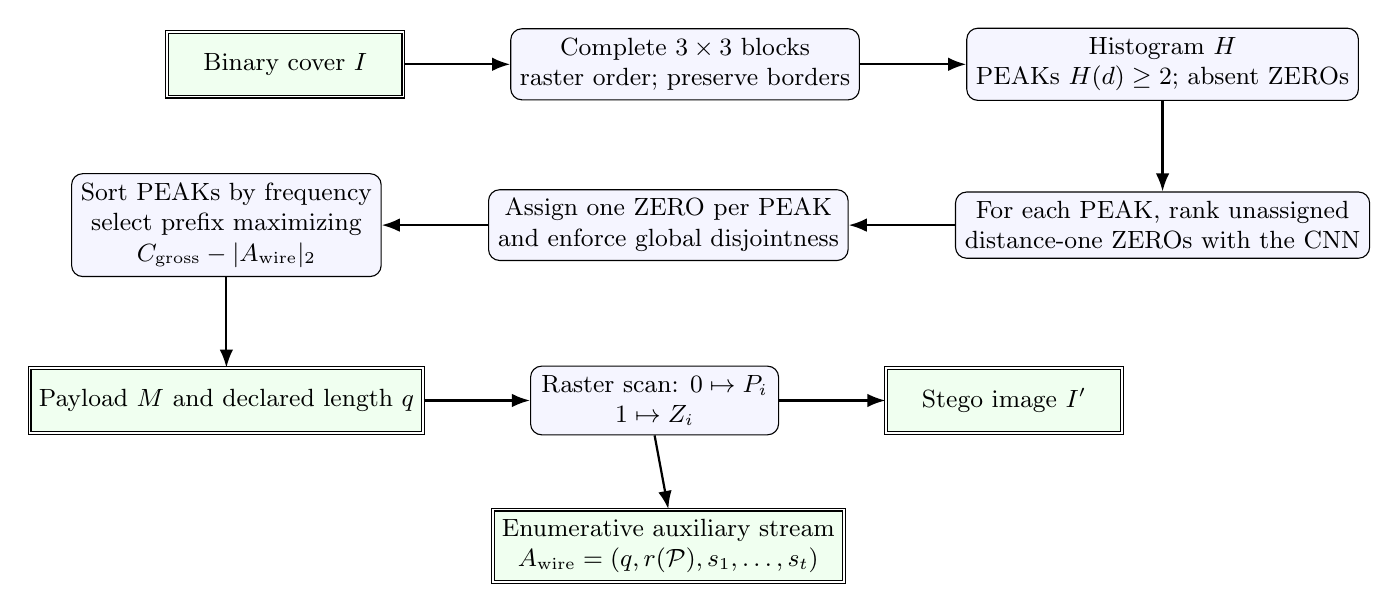
\begin{tikzpicture}[
    node distance=1.15cm and 1.35cm,
    every node/.style={font=\small},
    process/.style={rectangle, draw, rounded corners, align=center,
      minimum width=3.15cm, minimum height=0.82cm, fill=blue!4},
    decision/.style={diamond, draw, aspect=2.2, align=center,
      inner sep=1pt, fill=orange!8},
    data/.style={rectangle, draw, double, align=center,
      minimum width=3.0cm, minimum height=0.82cm, fill=green!6},
    arrow/.style={-{Latex[length=2.3mm]}, thick}
]
\node[data] (input) {Binary cover $I$};
\node[process, right=of input] (partition) {Complete $3\times3$ blocks\\raster order; preserve borders};
\node[process, right=of partition] (hist) {Histogram $H$\\PEAKs $H(d)\ge2$; absent ZEROs};
\node[process, below=of hist] (rank) {For each PEAK, rank unassigned\\distance-one ZEROs with the CNN};
\node[process, left=of rank] (inject) {Assign one ZERO per PEAK\\and enforce global disjointness};
\node[process, left=of inject] (net) {Sort PEAKs by frequency\\select prefix maximizing\\$C_{\rm gross}-|A_{\rm wire}|_2$};
\node[data, below=of net] (message) {Payload $M$ and declared length $q$};
\node[process, right=of message] (embed) {Raster scan: $0\mapsto P_i$\\$1\mapsto Z_i$};
\node[data, right=of embed] (stego) {Stego image $I'$};
\node[data, below=of inject, yshift=-2.0cm] (wire) {Enumerative auxiliary stream\\$A_{\rm wire}=(q,r(\mathcal P),s_1,\ldots,s_t)$};

\draw[arrow] (input) -- (partition);
\draw[arrow] (partition) -- (hist);
\draw[arrow] (hist) -- (rank);
\draw[arrow] (rank) -- (inject);
\draw[arrow] (inject) -- (net);
\draw[arrow] (net) -- (message);
\draw[arrow] (message) -- (embed);
\draw[arrow] (embed) -- (stego);
\draw[arrow] (embed.south) -- (wire.north);
\end{tikzpicture}
}
\caption{Evaluated embedding pipeline. Learned distance-one assignment is
followed by explicit net-capacity optimization and enumerative serialization
within a reversible-data-hiding synchronization model.}
\label{fig:embedding-flow}
\end{figure*}

\begin{algorithm*}[t]
\caption{Net-Aware CNN-Ranked Distance-One Embedding}
\label{alg:embedding}
\begin{algorithmic}[1]
\Require Binary image $I$, payload $M=(m_1,\ldots,m_q)$, trained ranker $f_\theta$
\Ensure Stego image $I'$, serialized auxiliary stream $A_{\rm wire}$
\State Enumerate complete $3\times3$ blocks and compute $H(d)$
\State $\mathcal P_0\gets\{d:H(d)\ge2,\ d\notin\{0,511\}\}$; sort by $(-H(d),d)$
\State $\mathcal Z\gets\{d:H(d)=0\}$; $\mathcal U\gets\emptyset$; $\mathcal T\gets\emptyset$
\For{each $P_i\in\mathcal P_0$}
    \State $\mathcal C_i\gets\{Z\in\mathcal Z\setminus\mathcal U:D(P_i,Z)=1\}$
    \If{$\mathcal C_i\neq\emptyset$}
        \State $Z_i\gets\arg\min_{Z\in\mathcal C_i}(f_\theta(I,P_i,Z),Z)$
        \State $\mathcal T[P_i]\gets\{0\mapsto P_i,1\mapsto Z_i\}$;
        $\mathcal U\gets\mathcal U\cup\{Z_i\}$
    \EndIf
\EndFor
\State Select the frequency-ordered prefix $\mathcal T^\star$ maximizing
$\sum_{P_i\in\mathcal T^\star}H(P_i)-|A_{\rm wire}(\mathcal T^\star)|_2$
\If{$q>\sum_{P_i\in\mathcal T^\star}H(P_i)$}
    \State reject the requested payload
\EndIf
\State $I'\gets I$; $j\gets1$
\For{each complete block of $I$ in raster order}
    \If{its pattern is $P_i\in\mathcal T^\star$ and $j\le q$}
        \State replace it by $\mathcal T^\star[P_i][m_j]$; $j\gets j+1$
    \EndIf
\EndFor
\State Serialize $q$, the active PEAK subset rank, and base-9 flip positions
\State \Return $I'$, $A_{\rm wire}$
\end{algorithmic}
\end{algorithm*}

\subsection{Efficient Extraction and Restoration}
\RevisionAddBegin
Extraction is designed as the exact inverse of the embedding contract, using
the marked image and the serialized auxiliary stream. The auxiliary stream
is decoded first because it fixes three pieces of synchronization information:
the payload length, the active PEAK subset, and the single flip position that
reconstructs each assigned ZERO. The decoder uses the serialized tables
directly, making the transmitted synchronization contract the source of
recovery decisions.

Once the active tables are reconstructed, they are collapsed into a single
inverse dictionary. This is possible because the encoder enforces global
injectivity: every stego pattern used by the codec belongs to at most one active
mapping. Therefore, observing a PEAK pattern decodes bit 0 and restores the same
PEAK, while observing its assigned ZERO decodes bit 1 and is also restored to
the PEAK. Patterns outside the dictionary are copied unchanged. This dictionary
view turns extraction into one linear raster scan with constant-time lookup.

The serialized payload length provides the stopping condition. After $q$ bits
have been recovered, remaining blocks are left unchanged because embedding used
the same declared stopping point. If the scan finishes before $q$ bits
are recovered, the pair $(I',A_{\rm wire})$ is rejected as inconsistent. This
explicit rejection rule is necessary because exact reversibility is guaranteed
for matched marked-image and auxiliary-stream pairs transmitted over a lossless
channel.

\RevisionAddEnd
\begin{figure*}[t]
\centering
\resizebox{\textwidth}{!}{
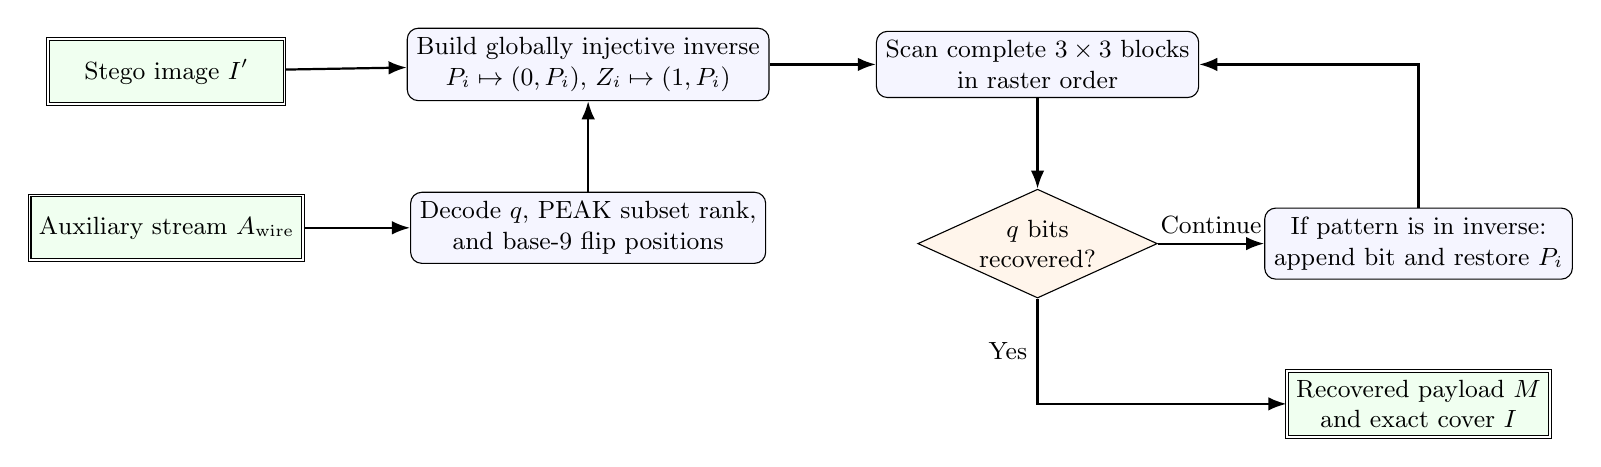
\begin{tikzpicture}[
    node distance=1.15cm and 1.35cm,
    every node/.style={font=\small},
    process/.style={rectangle, draw, rounded corners, align=center,
      minimum width=3.15cm, minimum height=0.82cm, fill=blue!4},
    decision/.style={diamond, draw, aspect=2.2, align=center,
      inner sep=1pt, fill=orange!8},
    data/.style={rectangle, draw, double, align=center,
      minimum width=3.0cm, minimum height=0.82cm, fill=green!6},
    arrow/.style={-{Latex[length=2.3mm]}, thick}
]
\node[data] (stego) {Stego image $I'$};
\node[data, below=of stego] (wire) {Auxiliary stream $A_{\rm wire}$};
\node[process, right=of wire] (decode) {Decode $q$, PEAK subset rank,\\and base-9 flip positions};
\node[process, above=of decode] (inverse) {Build globally injective inverse\\$P_i\mapsto(0,P_i)$, $Z_i\mapsto(1,P_i)$};
\node[process, right=of inverse] (scan) {Scan complete $3\times3$ blocks\\in raster order};
\node[decision, below=of scan] (done) {$q$ bits\\recovered?};
\node[process, right=of done] (lookup) {If pattern is in inverse:\\append bit and restore $P_i$};
\node[data, below=of lookup] (outputs) {Recovered payload $M$\\and exact cover $I$};
\draw[arrow] (stego) -- (inverse);
\draw[arrow] (wire) -- (decode);
\draw[arrow] (decode) -- (inverse);
\draw[arrow] (inverse) -- (scan);
\draw[arrow] (scan) -- (done);
\draw[arrow] (done) -- node[above]{Continue} (lookup);
\draw[arrow] (lookup) |- (scan);
\draw[arrow] (done.south) |- node[pos=0.25,left]{Yes} (outputs.west);
\end{tikzpicture}
}
\caption{Extraction and restoration pipeline. The serialized payload length
provides an unambiguous stopping condition, and incomplete border blocks remain
untouched.}
\label{fig:extraction-flow}
\end{figure*}

To reduce extraction complexity, all mapping tables are merged into a single inverse dictionary:
\begin{equation}
\mathcal{D} : p \mapsto (m, P_i),
\label{eq:inverse-dictionary}
\end{equation}
where $p$ is a stego pattern, $m\in\{0,1\}$ the extracted bit, and $P_i$ the
original pattern.

\begin{algorithm*}[t]
\caption{Deterministic Extraction and Exact Restoration}
\label{alg:extraction}
\begin{algorithmic}[1]
\Require Stego image $I'$, serialized auxiliary stream $A_{\rm wire}$
\Ensure Extracted message $M$, restored image $I$
\State Decode payload length $q$, active PEAKs, and their flip positions
\State Reconstruct all tables $T_i=\{0\mapsto P_i,1\mapsto Z_i\}$
\State Build $\mathcal D[P_i]=(0,P_i)$ and $\mathcal D[Z_i]=(1,P_i)$
\State $I\gets I'$; $M\gets\emptyset$
\For{each complete block of $I'$ in raster order}
    \If{$|M|=q$}
        \State \textbf{break}
    \EndIf
    \State Compute pattern index $d$
    \If{$d \in \mathcal{D}$}
        \State Append the decoded bit to $M$ and replace the block by its PEAK
    \EndIf
\EndFor
\If{$|M|\neq q$}
    \State reject the inconsistent stego/auxiliary pair
\EndIf
\State \Return $M$, $I$
\end{algorithmic}
\end{algorithm*}

\subsection{Learned Ranking, Ablations, and Wire Accounting}

\subsubsection*{Distortion characteristics}

For each embedded block mapped from $P_i$ to $\mathcal{Z}_i$, the number of flipped pixels is bounded by:
\begin{equation}
\max_{Z_j \in \mathcal{Z}_i} D_{i,j},
\label{eq:distortion-bound}
\end{equation}
ensuring pattern-specific distortion control.

\subsubsection*{Gaussian-process diagnostic}
\label{subsec:param_optim}

The parameter $\alpha$ is explored by Gaussian-process Bayesian optimization.
For every evaluated value, the implementation records capacity, PSNR, DRD, and
the normalized objective
\begin{equation}
J(\alpha)=\lambda\left(1-\frac{C_{\text{total}}(\alpha)}{C_{\mathrm{ref}}}\right)
+(1-\lambda)\mathrm{DRD}(\alpha).
\label{eq:gp-objective}
\end{equation}
Expected Improvement selects the next value of $\alpha$
\cite{Frazier2018Bayesian}. The equal weighting
$\lambda=0.5$ gives the two normalized diagnostic terms identical influence;
\RevisionAddBegin
it serves only the exploratory scalarization of the unconstrained diagnostic.
A $\lambda$ sweep therefore characterizes the exploration stage, whereas all
final tables use the independently specified distance-one policy. Optimizing
$\alpha$ alone provides incomplete control of
\RevisionAddEnd
$\mathrm{DRD}<1$, motivating the constrained distance-one policy used by the
integrated system. The exploratory search uses
$\alpha\in[0,1.5]$, initial points $\{0,0.5,1,1.5\}$, six EI iterations on a
\RevisionAddBegin
151-point grid, $\lambda=0.5$, exploration 0.01, and a Mat\'ern-$5/2$ kernel
\RevisionAddEnd
with a white-noise term. The random seed is 20260607.

\subsubsection*{CNN-based candidate ranking}

For a PEAK pattern and each distance-one ZERO candidate, the CNN receives three
\RevisionAddBegin
$9\times9$ channels: the centered PEAK, the centered candidate, and the average
\RevisionAddEnd
spatial context of all PEAK occurrences. It regresses the empirical
reciprocal-distance replacement cost. The candidate with the smallest predicted
\RevisionAddBegin
cost is assigned to symbol 1, while symbol 0 preserves the PEAK.
\RevisionAddEnd

The $9\times9$ support covers the central $3\times3$ block and a three-pixel
margin in every direction. It contains the complete $5\times5$ DRD support
around each of the nine possible flipped pixels, including pixels outside the
\RevisionAddBegin
embedding block; a $7\times7$ patch covers corner flips only partially.
Larger patches add context beyond the local training target.
\RevisionAddEnd

The network contains two $3\times3$ convolutional layers with 16 and 32
channels and ReLU activations, adaptive $3\times3$ average pooling, and a
$288\rightarrow64\rightarrow1$ regressor with ReLU and Softplus. Training uses
Smooth-L1 loss, AdamW with learning rate $10^{-3}$, batch size 128, 20 epochs,
\RevisionAddBegin
and seed 20260607. Complete source images define the train/validation split at
image level.
\RevisionAddEnd

Figure~\ref{fig:cnn-architecture} summarizes the evaluated architecture and
its scalar candidate-cost output.

\begin{figure*}[t]
\centering
\resizebox{\textwidth}{!}{
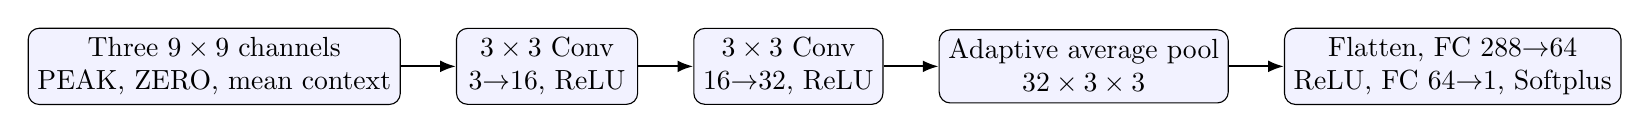
\begin{tikzpicture}[
  node distance=0.7cm,
  layer/.style={rectangle,draw,rounded corners,align=center,
    minimum height=0.75cm,minimum width=2.3cm,fill=blue!5},
  arrow/.style={-{Latex[length=2mm]},thick}
]
\node[layer] (input) {Three $9\times9$ channels\\PEAK, ZERO, mean context};
\node[layer, right=of input] (conv1) {$3\times3$ Conv\\3$\rightarrow$16, ReLU};
\node[layer, right=of conv1] (conv2) {$3\times3$ Conv\\16$\rightarrow$32, ReLU};
\node[layer, right=of conv2] (pool) {Adaptive average pool\\$32\times3\times3$};
\node[layer, right=of pool] (reg) {Flatten, FC 288$\rightarrow$64\\ReLU, FC 64$\rightarrow$1, Softplus};
\draw[arrow] (input) -- (conv1);
\draw[arrow] (conv1) -- (conv2);
\draw[arrow] (conv2) -- (pool);
\draw[arrow] (pool) -- (reg);
\end{tikzpicture}}
\caption{Candidate-cost CNN used to rank globally available distance-one ZERO
patterns. The scalar output estimates reciprocal-distance replacement cost.}
\label{fig:cnn-architecture}
\end{figure*}

\subsubsection*{Random-Forest uniform-block ablation}
\label{subsec:rf-layer}

Uniform blocks are processed by a second reversible layer. A Random Forest
classifier predicts whether a block admits a low-cost single-pixel flip from
its $9\times9$ context, and a second forest predicts the pixel position. The
\RevisionAddBegin
safety label uses a local reciprocal-distance cost at most 0.5.
\RevisionAddEnd
Selected coordinates and positions are compactly serialized for exact
extraction and restoration. The experiment shows that the classifier
identifies reliable locations, while the coordinate stream defines the next
compression target. The final net-aware configuration therefore assigns its
bit budget to the enumerative block-mapping layer.

Both forests use 120 trees and maximum depth 14. The safety model uses
minimum leaf size 2 and balanced class weights; the position model uses
minimum leaf size 1. Validation is grouped by source image with three folds,
seed 20260607, and a deployment probability threshold of 0.7. These bounded
defaults were fixed before the net-capacity evaluation: 120 trees stabilize
the grouped predictions, depth 14 limits memorization of image-specific
contexts, and the 0.7 threshold favors precision when every accepted block
\RevisionAddBegin
incurs coordinate overhead. They were fixed before evaluating the reported
test outcomes. This layer is an evaluated ablation, and the final payload
figures focus on the enumerative block-mapping layer because the current
coordinate stream outweighs the measured gross gain.
\RevisionAddEnd

\subsubsection*{Net-capacity accounting}

Useful capacity subtracts the exact serialized side information:
\begin{equation}
C_{\mathrm{net}}=C_{\mathrm{gross}}-|A_{\mathrm{wire}}|_2.
\label{eq:net-capacity}
\end{equation}
For distance-one mappings, the wire format ranks the sorted active-PEAK subset
in the combinatorial number system. The corresponding nine possible flip
\RevisionAddBegin
positions are then represented as base-9 digits. This representation closely
matches the information content of the mapping set and is more compact than
independent fixed-width pairs. Mapping pairs are ordered by occurrence count,
and the net-maximizing prefix is retained. When every subset has nonpositive
useful capacity, the encoder returns the unchanged image.
\RevisionAddEnd

For $t$ active PEAKs $0\le p_1<\cdots<p_t<512$, the subset rank is
\begin{equation}
r(\mathcal P)=\sum_{j=1}^{t}\binom{p_j}{j}.
\label{eq:combination-rank}
\end{equation}
If $s_j\in\{0,\ldots,8\}$ is the flipped bit position, the combined integer is
\begin{equation}
u=r(\mathcal P)9^t+\sum_{j=1}^{t}s_j9^{t-j}.
\label{eq:enumerative-state}
\end{equation}
For example, with active PEAKs $\{5,9,12\}$ and flip positions $(0,4,8)$,
$r=\binom51+\binom92+\binom{12}3=261$, the base-9 component is 44, and the
combined state is $u=261\times9^3+44=190313$.
The wire stream contains a one-byte raw/compressed marker, a four-byte magic
identifier, a one-byte format version, the 32-bit big-endian payload length
$q$, the 16-bit big-endian table count $t$, and the shortest big-endian byte
string capable of representing the joint state space
$\binom{512}{t}9^t$. Thus the variable state is charged as
\begin{equation}
8\left\lceil
\frac{\left\lceil\log_2\left(\binom{512}{t}9^t\right)\right\rceil}{8}
\right\rceil
\label{eq:wire-state-bytes}
\end{equation}
bits, and the fixed ABM header is 96 bits. The active PEAKs are sorted by
increasing pattern index inside the combinatorial rank, while the
frequency-ordered prefix determines which PEAKs are active. Image dimensions
are provided by the stego container and are checked by the extraction API. The
stream is a serialized plaintext synchronization channel; confidentiality and
authentication, when required by an application, are orthogonal transport-layer
services.

Table~\ref{tab:wire-model} gives the executable synchronization model used in
the comparisons. For ABM the listed representation is part of the proposed
codec. For baselines, the original publications specify the reversible
principle and some parameters while leaving the complete independent byte
stream open; the table therefore records the conservative executable
representations implemented for this protocol.

\begin{table*}[t]
\centering
\caption{Executable auxiliary-information model used for exact extraction and
restoration.}
\label{tab:wire-model}
\resizebox{\textwidth}{!}{
\begin{tabular}{@{}lllll@{}}
\toprule
\textbf{Method} & \textbf{Auxiliary element} &
\textbf{Specified in cited paper} & \textbf{Executable representation} &
\textbf{Charged bits} \\
\midrule
ABM & Encoding marker & Proposed codec & raw/compressed marker byte & 8 \\
ABM & Stream identity & Proposed codec & magic and version bytes & 40 \\
ABM & Payload length $q$ & Proposed codec & big-endian uint32 & 32 \\
ABM & Active table count $t$ & Proposed codec & big-endian uint16 & 16 \\
ABM & Active PEAKs and flips & Proposed codec &
byte-aligned joint state in Eq.~\ref{eq:wire-state-bytes} & variable \\
Huynh--Nguyen & Peak, selected states, $q$ & Partial & compact byte stream with zlib option & measured \\
Dong & Context divisor, end position, $q$, PF/PFR map & Partial &
packed and zlib-compressed location map & measured \\
PPOCP & Pair level, used centers, original centers, $q$ & Partial &
varint positions plus bit-packed original centers & measured \\
\bottomrule
\end{tabular}}
\vspace{2pt}
{\footnotesize\RaggedRight Image dimensions are supplied by the marked-image container for ABM
and checked by the decoder API. Baseline synchronization formats are treated
as conservative executable formats for the common round-trip protocol.\par}
\end{table*}

\subsection{Comparison with Conventional Block-Mapping}

\RevisionAddBegin
Huynh--Nguyen \cite{Huynh2025BlockMapping} is the closest direct
$3\times3$ PEAK/ZERO block-mapping comparator. The comparison therefore
isolates one difference: the block representation, the PEAK/ZERO idea, and
Hamming-distance control are established foundations, while the evaluated
change is serialization-aware activation. The same reversible mapping family is
retained when its exact encoded description leaves useful payload after
Equation~\ref{eq:net-capacity}. On the eight document benchmarks, the proposed
implementation provides 2874 gross bits and 2245 net bits on average after 629
auxiliary bits are charged. Huynh--Nguyen report 2070 gross bits under their
own protocol; this published value is contextual because
their serialized auxiliary cost remains open.
\RevisionAddEnd

\subsection{Computational Complexity and Formal Properties}
\label{subsec:complexity-analysis}

\RevisionAddBegin
The following propositions summarize the asymptotic cost and recovery
guarantees of the deployed embedding and extraction algorithms. The analysis
uses the finite 512-state $3\times3$ alphabet to show that histogram, mapping,
and inverse-dictionary structures remain constant with respect to image size,
while image traversal dominates runtime. The final propositions establish
deterministic reversibility and block independence.
\RevisionAddEnd

\paragraph{Notation.}
Let $n=MN$ denote the total number of pixels and
$B=\lfloor M/3\rfloor\lfloor N/3\rfloor$ the number of complete
$3\times3$ blocks.
Let $\mathcal{P}$ be the set of frequent (PEAK) patterns and
$\mathcal{Z}$ the set of unused (ZERO) patterns.
For a pattern $P_i \in \mathcal{P}$, let $n_i$ be the number of blocks
exhibiting $P_i$, $L_i$ the embedding capacity associated with $P_i$, and
$E = \sum_i n_i^{\text{emb}}$ the total number of blocks actually used for
embedding.

\begin{proposition}[Embedding Time Complexity]
The time complexity of the deployed distance-one embedding algorithm is
\begin{equation}
O\!\left(n+|\mathcal P_0|\,c_\theta+E\right)=O(n),
\label{eq:embedding-complexity}
\end{equation}
where $c_\theta$ is the fixed cost of evaluating at most nine candidates with
the fixed CNN.
\end{proposition}

\begin{proof}
The algorithm first partitions the image into blocks and computes pattern
indices, which requires a single pass over all pixels and thus $O(n)$ time.
Histogram construction and pattern classification are performed in constant
time per block, yielding $O(B)=O(n)$ complexity.
For each PEAK, its at most nine distance-one neighbors are generated directly
and ranked by the fixed-size CNN, requiring
$O(|\mathcal P_0|c_\theta)$ time. Since the binary $3\times3$ pattern space
contains only 512 states, this term is bounded independently of image size.
Finally, each embedding operation consists of a constant-time table lookup and
block substitution, and is executed for $E$ blocks, contributing $O(E)$ time.
Summing all terms gives the stated complexity.
\end{proof}

\begin{proposition}[Embedding Space Complexity]
The space complexity of the embedding algorithm is
\begin{equation}
O(n+q).
\label{eq:embedding-space}
\end{equation}
\end{proposition}

\begin{proof}
The algorithm stores the original and modified images, requiring $O(n)$ space.
The histogram, mapping tables, and inverse dictionary contain at most 512
states and therefore require constant space with respect to image size. The
payload buffer requires $O(q)$ space.
\end{proof}

\begin{proposition}[Optimized Extraction Time Complexity]
The optimized extraction algorithm runs in
\begin{equation}
O(n)
\label{eq:extraction-time}
\end{equation}
time.
\end{proposition}

\begin{proof}
Extraction scans the stego image once to reconstruct blocks and compute pattern
indices, which requires $O(n)$ time.
The inverse dictionary has at most 512 entries. Each complete block is
processed at most once in deterministic raster order with constant-time
lookup, and extraction stops after the declared $q$ bits.
\end{proof}

\begin{proposition}[Extraction Space Complexity]
The space complexity of the optimized extraction algorithm is
\begin{equation}
O(n+q).
\label{eq:extraction-space}
\end{equation}
\end{proposition}

\begin{proof}
During extraction, memory is required for the stego image, the recovered image,
and the inverse dictionary constructed from the mapping tables.
The inverse dictionary is bounded by the 512-state pattern alphabet, and the
message buffer stores exactly $q$ recovered bits.
\end{proof}

\begin{proposition}[Deterministic Reversibility]
Given an unmodified stego image and its valid auxiliary stream, the proposed
embedding and extraction procedures recover the payload and cover exactly.
\end{proposition}

\begin{proof}
Each table maps 0 to its PEAK and 1 to one absent distance-one pattern.
Assigned ZEROs are globally disjoint and were absent from the cover, so the
union of table ranges is injective. During extraction, the inverse dictionary
therefore maps every active stego pattern to one bit and one original PEAK.
Since blocks are non-overlapping, modified at most once, and processed in a
deterministic traversal order, the declared payload length gives a unique
stopping point. Unused complete blocks and incomplete border pixels are never
modified. Hence both the embedded message and original image are reconstructed
exactly.
\end{proof}

\begin{proposition}[Independent Blocks]
Embedding operations on distinct blocks are independent.
\end{proposition}

\begin{proof}
Each block is processed independently using a pattern-specific mapping table.
\RevisionAddBegin
Each operation is confined to the current block and uses the block's own state.
Therefore, embedding decisions are local and preserve inter-block independence.
\RevisionAddEnd
\end{proof}


\section{Experimental Evaluation}
\label{sec:experimental}

\subsection{Datasets, Splits, and Reproducibility}

The evaluation has two complementary scales. The eight standard
$512\times512$ binary document images used by Huynh--Nguyen
\cite{Huynh2025BlockMapping} support
direct validation against the block-mapping literature; their diversity is
shown in Figure~\ref{fig:dataset-final}. BOSSbase~\cite{Bas2011BOSS} provides
10,000 grayscale
images, from which seed 20260608 selects 100 profile images and 100 disjoint
\RevisionAddBegin
test images. The profile split supplies the image-level statistics needed by
the conservative Dong implementation. Test images are binarized at
\RevisionAddEnd
threshold 128. The CNN ranker trained on the document images is transferred
\RevisionAddBegin
directly to BOSSbase, preventing test-set adaptation.
\RevisionAddEnd

\begin{figure*}[t]
\centering
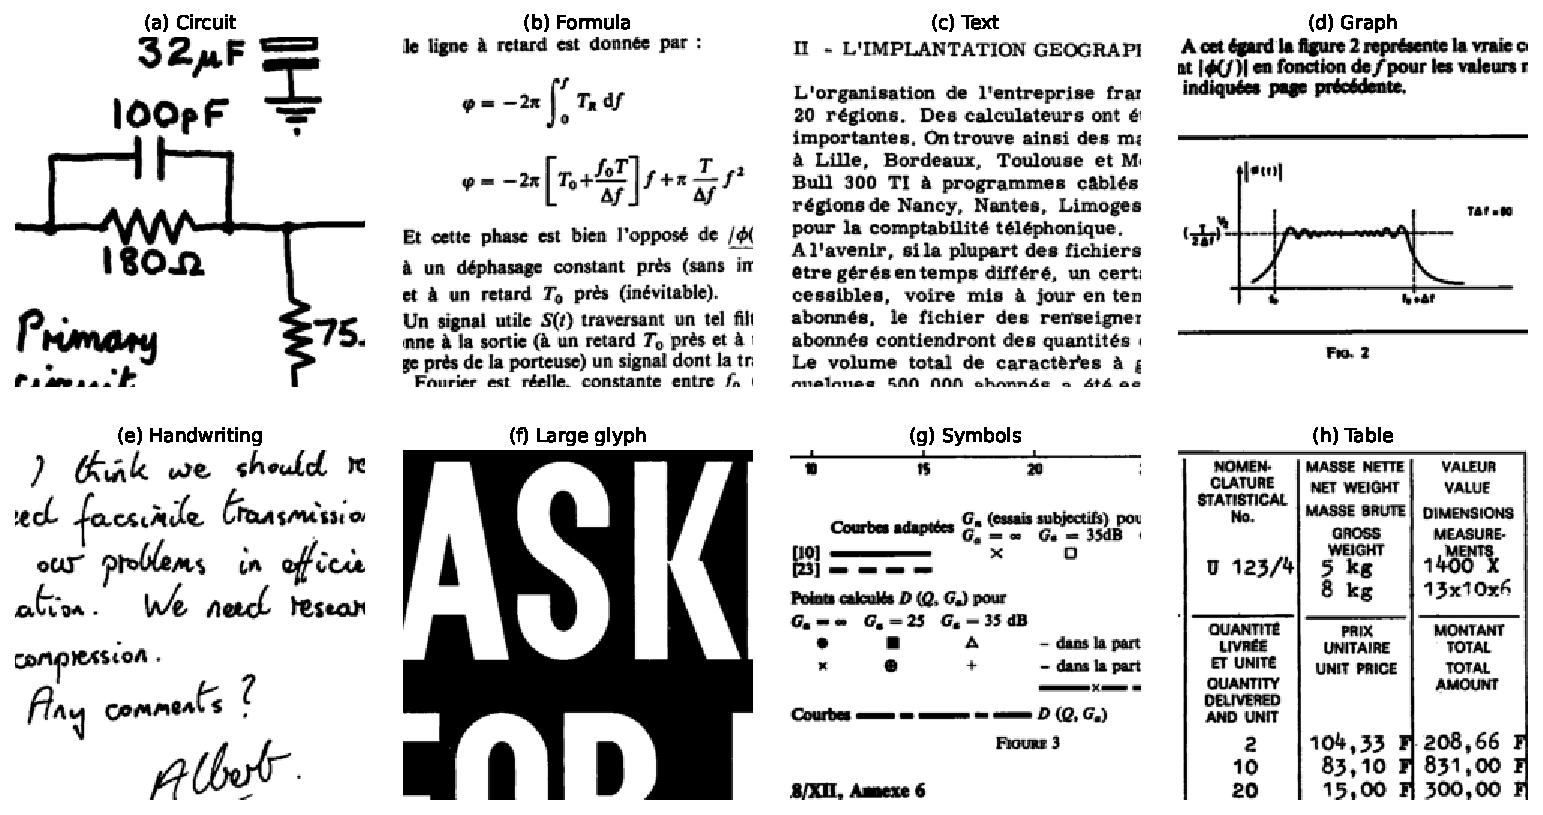
\includegraphics[width=\textwidth]{images/Figure_4.pdf}
\caption{Eight binary document images used for block-mapping validation.}
\label{fig:dataset-final}
\end{figure*}

The four-method protocol embeds identical pseudorandom messages at targets 64,
\RevisionAddBegin
128, 256, and 512 bits. A run counts as available after exact message
extraction and bitwise cover restoration. Huynh--Nguyen uses the
\RevisionAddEnd
published threshold $T=5$. Dong evaluates all context divisors
$l\in\{1,\ldots,10\}$ and retains the exact minimum-DRD result. PPOCP and Dong
use conservative serialized synchronization or location information where the
\RevisionAddBegin
publications leave the independent wire representation open. Accordingly,
\RevisionAddEnd
net-payload conclusions apply to the executable wire formats defined in this
\RevisionAddBegin
study, while DRD and availability provide a comparison less sensitive to
byte-stream conventions.
\RevisionAddEnd

\subsection{Metrics and Statistical Protocol}

Gross payload is the message length, auxiliary bits are the exact serialized
wire length, and useful payload is
\RevisionAddBegin
$C_{\mathrm{net}}=C_{\mathrm{gross}}-C_{\mathrm{aux}}$, where
$C_{\mathrm{aux}}=|A_{\mathrm{wire}}|_2$. Distortion is measured
with changed pixels, PSNR, and DRD \cite{Lu2004DRD}. Availability is the fraction of
\RevisionAddEnd
test images that carry the target and complete the exact round trip.

Primary per-payload comparisons use common available images. A secondary fixed
cohort contains the 46 images on which all four methods are available at all
four payloads. ABM is paired with each baseline for net bits and DRD using the
Wilcoxon signed-rank test and Holm correction within each payload. Mean net
payload is accompanied by a 95\% percentile bootstrap interval with 10,000
image-level resamples and seed 20260608. Runtime includes embedding,
serialization, extraction, and verification. Memory is peak process RSS minus
pre-call RSS, sampled every 2 ms. Experiments used Python 3.13.5, NumPy 2.2.6,
PyTorch 2.8.0 CPU, scikit-learn 1.7.2, and SciPy 1.17.1 on 64-bit Windows with
12 logical processors.

\subsection{Serialization-Aware Activation Ablation}
\label{subsec:component-ablations}

Table~\ref{tab:activation-ablation} isolates the central algorithmic decision.
All variants use the same CNN distance-one candidate assignment; only active
table selection and exact wire charging differ. A0 reports gross payload before
wire cost and is therefore a gross-reporting diagnostic reference point. A1
charges the wire after activating all feasible tables. A2 is the proposed
serialization-aware activation, which selects the frequency-ordered prefix that
maximizes Equation~\ref{eq:net-capacity}. Relative to A1, A2 reduces auxiliary
information by 180 bits on average and raises mean net payload by 105.9 bits
(4.95\%) while preserving exact reversibility on all eight document images.

\begin{table*}[t]
\centering
\caption{Central ablation of serialization-aware mapping activation on the
eight document images. Values are means in bits except DRD; the post-hoc value
in A0 is the net payload obtained when the exact wire is charged after the
gross-only selection.}
\label{tab:activation-ablation}
\resizebox{\textwidth}{!}{
\begin{tabular}{@{}llcrrrrr@{}}
\toprule
\textbf{Variant} & \textbf{Active-table selection} & \textbf{Wire charged} &
\textbf{Gross cap.} & \textbf{Payload} & \textbf{Aux.} &
\textbf{Net payload} & \textbf{Mean DRD} \\
\midrule
A0 & all feasible; gross reported & Gross only & 3932 & 2948 & 0
& 2948 (2139 post hoc) & 0.771 \\
A1 & all feasible; wire charged & Charged & 3932 & 2948 & 809
& 2139 & 0.778 \\
A2 proposed & serialized-net prefix & Charged & 3832 & 2874 & 629
& 2245 & 0.761 \\
\bottomrule
\end{tabular}}
\end{table*}

\subsection{Candidate Ranking and CNN Architecture}

Table~\ref{tab:ranker-ablation} compares the learned ranker with simple
non-learning alternatives under the same admissible distance-one ZERO set and
common payload per image. The CNN is close to the direct DRD-cost ranker and
improves mean DRD by about 5\% relative to Hamming-index ordering. The
reversible mechanism remains the deterministic, globally injective PEAK/ZERO
substitution defined in
Section~\ref{sec:proposedmethod}.

\begin{table}[t]
\centering
\caption{Ranker ablation with identical distance-one candidates and common
payloads.}
\label{tab:ranker-ablation}
\begin{tabular}{@{}lrrr@{}}
\toprule
\textbf{Ranker} & \textbf{Mean net} & \textbf{Mean DRD} &
\textbf{Round trip} \\
\midrule
Hamming index & 2141 & 0.822 & Exact \\
Direct DRD cost & 2139 & 0.778 & Exact \\
Transition preserving & 2140 & 0.829 & Exact \\
Connectivity aware & 2140 & 0.820 & Exact \\
CNN & 2137 & 0.780 & Exact \\
\bottomrule
\end{tabular}
\end{table}

Table~\ref{tab:cnn-architecture-ablation} gives the controlled CNN
architecture diagnostic. All configurations use 20 epochs, AdamW with learning
rate $10^{-3}$, Smooth-L1 loss, batch size 128, the same two-image
train/validation split, and deterministic seeds. The deployed two-layer
$9\times9$ model is retained as a compact compromise: it is close to the
lowest-MAE wider model, faster at inference, and keeps held-out placement DRD
within the same practical range.

\begin{table*}[t]
\centering
\caption{CNN architecture diagnostic on the two-image detailed split. Inference
time is measured on 4323 held-out candidates. Held-out DRD is the mean DRD
after model-ranked placement on the diagnostic held-out images. All
configurations share the reversible mapping and auxiliary stream.}
\label{tab:cnn-architecture-ablation}
\begin{tabular*}{\textwidth}{@{\extracolsep{\fill}}lrrrrrr@{}}
\toprule
\textbf{Configuration} & \textbf{Params} & \textbf{Train s} &
\textbf{Inf. $\mu$s} & \textbf{MAE} & \textbf{Pearson} &
\textbf{Held-out DRD} \\
\midrule
1 conv., $9\times9$, w24 & 14625 & 6.97 & 7.18 & 0.0716 & 0.962 & 0.848 \\
2 conv., $9\times9$, w24 & 38865 & 23.62 & 27.19 & 0.0339 & 0.991 & 0.830 \\
3 conv., $9\times9$, w24 & 44073 & 27.80 & 38.21 & 0.0347 & 0.991 & 0.848 \\
2 conv., $7\times7$, w24 & 38865 & 18.11 & 19.51 & 0.0383 & 0.989 & 0.845 \\
2 conv., $11\times11$, w24 & 38865 & 27.77 & 56.13 & 0.0485 & 0.985 & 0.825 \\
2 conv., $9\times9$, w16 & 23649 & 15.16 & 24.86 & 0.0379 & 0.990 & 0.839 \\
2 conv., $9\times9$, w32 & 56385 & 27.27 & 40.62 & 0.0303 & 0.992 & 0.847 \\
\bottomrule
\end{tabular*}
\end{table*}

\subsection{Serialization Sensitivity for Baselines}

The original descriptions of PPOCP, Dong, and Huynh--Nguyen specify the
reversible principles while leaving the complete standalone byte stream partly
unspecified. The common protocol therefore uses conservative executable
synchronization. We also ran a header-credit sensitivity check: for each
baseline, the method-identifying header, version field, and image-shape fields
are removed from the charged cost, giving a 104-bit credit while retaining the
payload-critical maps, states, locations, and payload length. With this
credited accounting, ABM retains the highest mean net payload on every
all-method matched cohort: $-57$ vs.\ $-120$ bits at 64, $-7$ vs.\ $-72$ bits
at 128, $93$ vs.\ $23$ bits at 256, and $309$ vs.\ $200$ bits at 512 for the
best credited baseline. This fixed-header variation leaves the useful-capacity
ordering unchanged for the tested executable representations.

\subsection{Machine-Learning Validation}

Image-wise leave-one-out (LOSO) validation trains eight independent CNNs, each
on seven document images and tests it on the remaining complete image. Across
13,808 held-out candidates, pooled mean absolute error is 0.0367 and pooled
Pearson correlation is 0.9893; per-image correlations range from 0.9861 to
0.9939. A separate LOSO placement experiment applies each fold model to its
held-out image at an identical 75\% distance-one payload. Mean DRD decreases
from 0.8054 with deterministic Hamming-index ordering to 0.7663 with CNN
ordering, a 4.85\% reduction. All eight images improve, with per-image
reductions from 2.83\% to 7.94\%, while every message and cover is recovered
\RevisionAddBegin
exactly. The separate two-image architecture diagnostic in
Table~\ref{tab:cnn-architecture-ablation} evaluates 4323 held-out candidates
under the fixed 20-epoch protocol. Thus, regression accuracy and operational
DRD impact are evaluated separately, with fold-level regression and placement
results provided with the reproducibility artifacts.
\RevisionAddEnd

The uniform-block Random Forest is evaluated by source-image-grouped
cross-validation on 14,798 samples. It reaches ROC AUC 0.995, precision 0.897,
\RevisionAddBegin
recall 0.970, and flip-position accuracy 0.971. In the combined reversible
pipeline, the layer adds 181.4 gross bits per document image on average, while
its current coordinate representation uses 2691.0 auxiliary bits. The
resulting combined net payload is therefore $-264.6$ bits on average, compared
with 2245.0 bits for the base enumerative block-mapping layer. This identifies
coordinate coding as a concrete optimization opportunity and keeps the Random
Forest layer as a diagnostic component.
\RevisionAddEnd

\subsection{Document-Image and External Net Capacity}

Table~\ref{tab:document-net} reports the integrated CNN-ranked mapping layer at
a 75\% payload budget. Auxiliary sizes are measured from serialized bytes, and
all eight messages and covers are recovered exactly.

\begin{table}[t]
\centering
\caption{Net-aware results on the eight binary document images.}
\label{tab:document-net}
\begin{tabular}{@{}lrrrr@{}}
\toprule
\textbf{Image} & \textbf{Gross} & \textbf{Aux.} & \textbf{Net} & \textbf{DRD} \\
\midrule
circuit-2 & 1576 & 592 & 984 & 0.583 \\
formula-5 & 3692 & 672 & 3020 & 0.900 \\
graph1-5 & 1978 & 632 & 1346 & 0.662 \\
handwr2-8 & 2351 & 632 & 1719 & 0.768 \\
large-8 & 1138 & 488 & 650 & 0.616 \\
symbol-6 & 2367 & 672 & 1695 & 0.897 \\
table1-3 & 4161 & 656 & 3505 & 0.789 \\
french-4 & 5729 & 688 & 5041 & 0.864 \\
\midrule
\textbf{Average} & \textbf{2874} & \textbf{629} & \textbf{2245} & \textbf{0.760} \\
\bottomrule
\end{tabular}
\end{table}

\RevisionAddBegin
On the 100 BOSSbase test images, net-aware table selection gives 669.6 gross,
377.1 auxiliary, and 292.5 net bits on average. Median net capacity is 159
bits, 75 images are net positive, mean DRD is 0.300, and every evaluated
message and cover is recovered exactly. Disabling net-aware table selection on
the same sample yields 832.5 gross, 731.4 auxiliary, and 101.1 net bits on
average, showing that the active-prefix decision also improves the external
transfer setting.
\RevisionAddEnd

\subsection{Multi-Payload Common-Protocol Results}

Table~\ref{tab:multiload} and Figure~\ref{fig:multiload} summarize the
all-method matched subsets. ABM moves from metadata-dominated operation at 64
bits to a median-positive point at 128 bits and a clearly positive operating
\RevisionAddBegin
region at 256 and 512 bits. PPOCP defines the lowest-DRD curve, while ABM
defines the highest-net curve.
\RevisionAddEnd

\begin{table*}[t]
\centering
\caption{Mean net bits and median DRD on all-method matched images.}
\label{tab:multiload}
\begin{tabular*}{\textwidth}{@{\extracolsep{\fill}}rrcccccccc@{}}
\toprule
& & \multicolumn{2}{c}{\textbf{Proposed ABM}} &
\multicolumn{2}{c}{\textbf{Dong}} &
\multicolumn{2}{c}{\textbf{Huynh--Nguyen}} &
\multicolumn{2}{c}{\textbf{PPOCP}} \\
\cmidrule(lr){3-4}\cmidrule(lr){5-6}\cmidrule(lr){7-8}\cmidrule(lr){9-10}
\textbf{Target} & \textbf{Matched} & \textbf{Net} & \textbf{DRD} &
\textbf{Net} & \textbf{DRD} & \textbf{Net} & \textbf{DRD} &
\textbf{Net} & \textbf{DRD} \\
\midrule
64  & 86 & $-57$ & 0.041 & $-224$ & 0.056 & $-2200$ & 0.035 & $-997$ & 0.023 \\
128 & 83 & $-7$  & 0.080 & $-176$ & 0.108 & $-2096$ & 0.070 & $-1653$ & 0.041 \\
256 & 69 & \textbf{93} & 0.135 & $-81$ & 0.200 & $-1812$ & 0.117 & $-2856$ & 0.064 \\
512 & 46 & \textbf{309} & 0.176 & 96 & 0.332 & $-1191$ & 0.178 & $-4822$ & 0.097 \\
\bottomrule
\end{tabular*}
\end{table*}

\begin{table*}[t]
\centering
\caption{Fixed-cohort sensitivity analysis on the 46 images available for
every method and payload. Values are mean net bits with 95\% bootstrap
intervals; DRD is the cohort median.}
\label{tab:fixed-cohort}
\resizebox{\textwidth}{!}{
\begin{tabular}{@{}rccc@{}}
\toprule
\textbf{Target} & \textbf{Method} & \textbf{Mean net bits (95\% CI)} &
\textbf{Median DRD}\\
\midrule
64 & Proposed ABM & $-48.5\;[-49.0,-48.0]$ & 0.022\\
   & Dong / Huynh--Nguyen / PPOCP & $-226.3\;[-229.6,-223.0]$ /
   $-1644.7\;[-1854.3,-1447.5]$ / $-1028.0\;[-1063.3,-990.1]$ &
   0.029 / 0.024 / 0.012\\
128 & Proposed ABM & $8.0\;[5.7,10.1]$ & 0.043\\
   & Dong / Huynh--Nguyen / PPOCP & $-178.3\;[-187.8,-169.9]$ /
   $-1582.8\;[-1792.4,-1386.8]$ / $-1707.8\;[-1767.5,-1643.0]$ &
   0.066 / 0.044 / 0.025\\
256 & Proposed ABM & $113.9\;[108.3,119.0]$ & 0.087\\
   & Dong / Huynh--Nguyen / PPOCP & $-83.8\;[-105.6,-65.7]$ /
   $-1456.3\;[-1656.2,-1260.9]$ / $-2954.1\;[-3060.2,-2835.8]$ &
   0.132 / 0.084 / 0.050\\
512 & Proposed ABM & $309.0\;[289.7,325.9]$ & 0.176\\
   & Dong / Huynh--Nguyen / PPOCP & $95.8\;[55.1,131.0]$ /
   $-1190.6\;[-1397.6,-996.7]$ / $-4821.7\;[-5025.6,-4607.1]$ &
   0.332 / 0.178 / 0.097\\
\bottomrule
\end{tabular}}
\end{table*}

Table~\ref{tab:fixed-cohort} preserves the ordering observed in the
payload-specific matched analysis. It also removes changing-cohort composition
as an explanation for the positive ABM net payload from 128 bits onward.

\begin{figure*}[t]
\centering
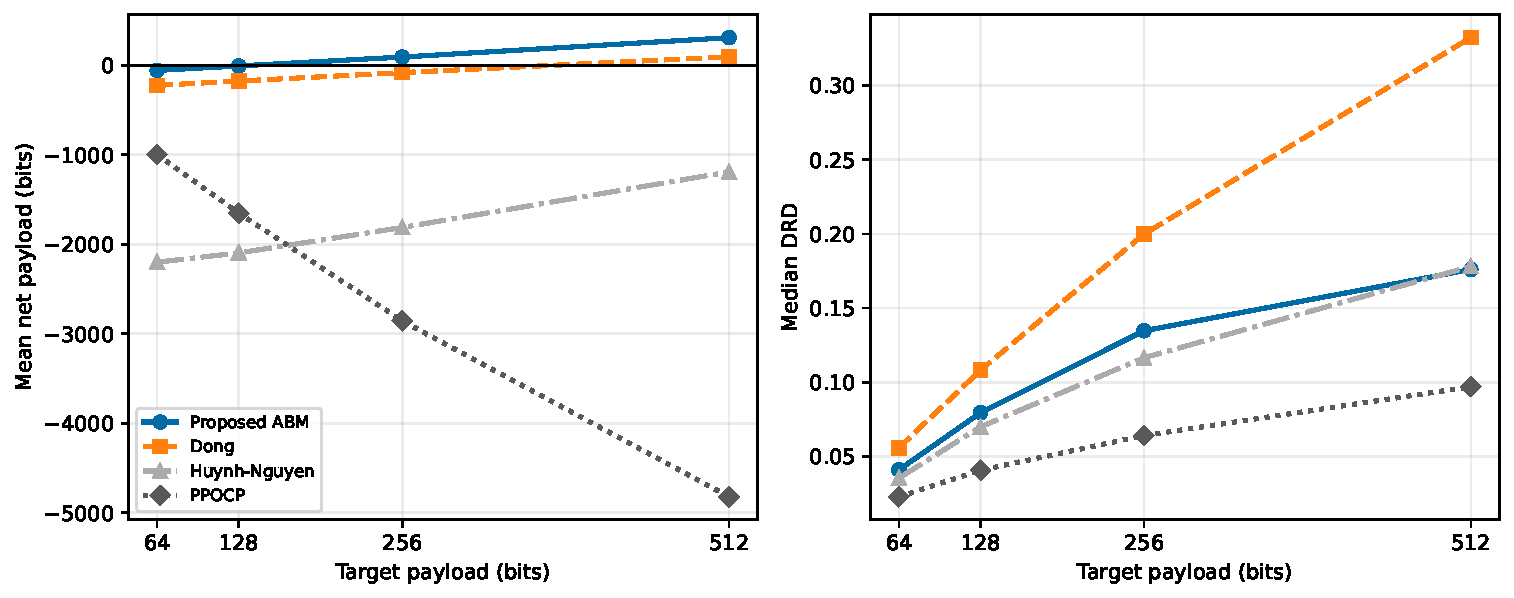
\includegraphics[width=\textwidth]{images/Figure_5.pdf}
\caption{Payload scaling on all-method matched images: mean net payload
(left) and median DRD (right), with 95\% bootstrap confidence bands.}
\label{fig:multiload}
\end{figure*}

Figure~\ref{fig:protocol-overview} complements the table with availability and
\RevisionAddBegin
the net-bits--DRD operating curves. PPOCP carries every target on all
\RevisionAddEnd
test images. ABM availability progresses from 89\% at 64 bits to 70\% at 512
bits, matching Dong at the highest target and remaining above Huynh--Nguyen.
\RevisionAddBegin
The right panel is descriptive because the methods span different DRD ranges;
Table~\ref{tab:fixed-cohort} provides the
\RevisionAddEnd
controlled cross-payload comparison.

\begin{figure*}[t]
\centering
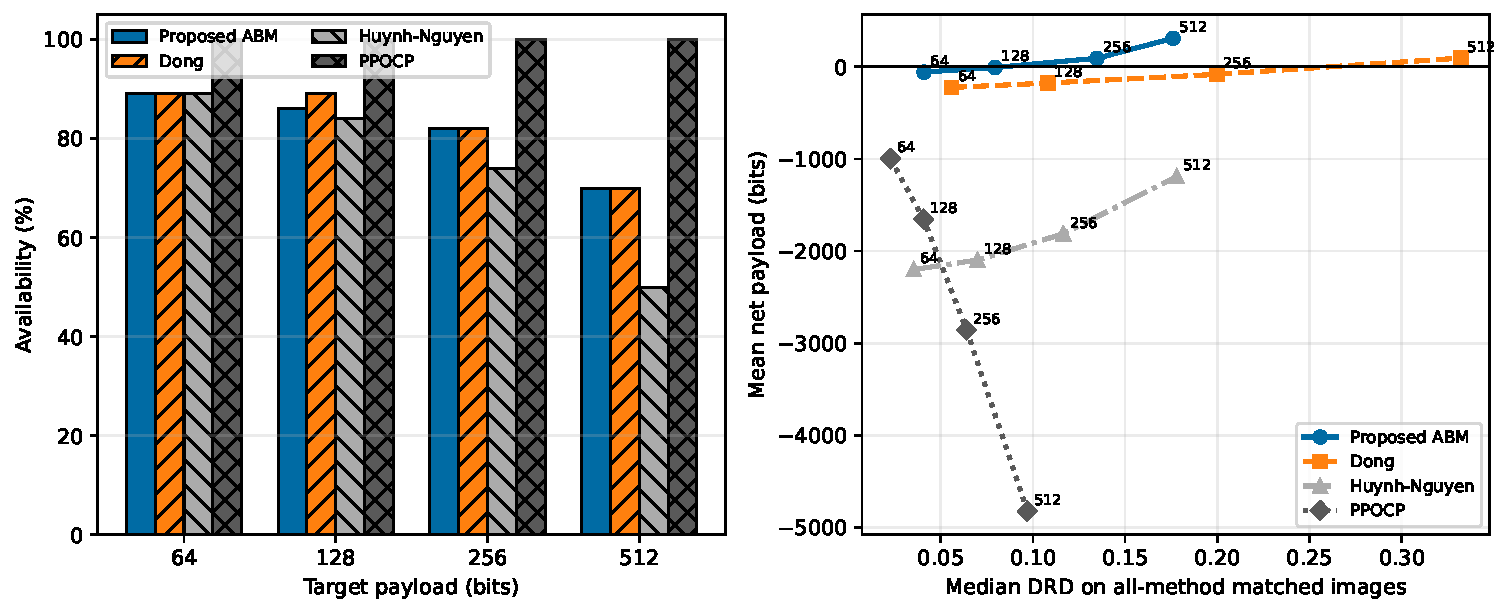
\includegraphics[width=\textwidth]{images/Figure_6.pdf}
\caption{Complementary views of payload feasibility and useful-capacity
efficiency. Error bars denote 95\% bootstrap confidence intervals for mean net
payload; numbers on the right panel denote target payloads in bits.}
\label{fig:protocol-overview}
\end{figure*}

\subsection{Paired Significance and Binarization Strata}

At each payload, ABM's paired net advantage over Dong, Huynh--Nguyen, and
PPOCP remains significant after Holm correction. At 256 bits, adjusted
$p$-values are below $6.7\times10^{-13}$, $3.1\times10^{-13}$, and
$2.2\times10^{-14}$, respectively. Median ABM net gains are 160, 1752, and
\RevisionAddBegin
3016 bits, with paired rank-biserial correlations of 0.974, 1.000, and 1.000.
DRD tests place ABM below Dong and above the perceptually focused PPOCP and
Huynh--Nguyen curves, yielding a two-objective interpretation.
\RevisionAddEnd

Binarization suitability is defined before embedding: threshold 128 must agree
with Otsu on at least 95\% of pixels, and foreground fraction must lie in
$[0.05,0.95]$. Twenty-two test images satisfy this criterion. As shown in
Figure~\ref{fig:binarization}, ABM is available on all 22 through 256 bits,
while net-positive behavior at 256 and 512 bits is present in both strata.
\RevisionAddBegin
Suitability therefore serves as an applicability indicator, with net
performance reported separately in both strata.
\RevisionAddEnd

At 512 bits, the 70 available images have mean foreground fraction 0.289,
189.2 eligible non-uniform PEAK patterns, and non-uniform $8\times8$ block
fraction 0.227. The 30 unavailable images have corresponding means 0.025,
\RevisionAddBegin
34.2, and 0.024. Unavailable cases are therefore concentrated in near-empty or
nearly uniform thresholded photographs with too few repeated non-uniform
patterns; available cases still restore the message and cover exactly.
\RevisionAddEnd

\begin{figure*}[t]
\centering
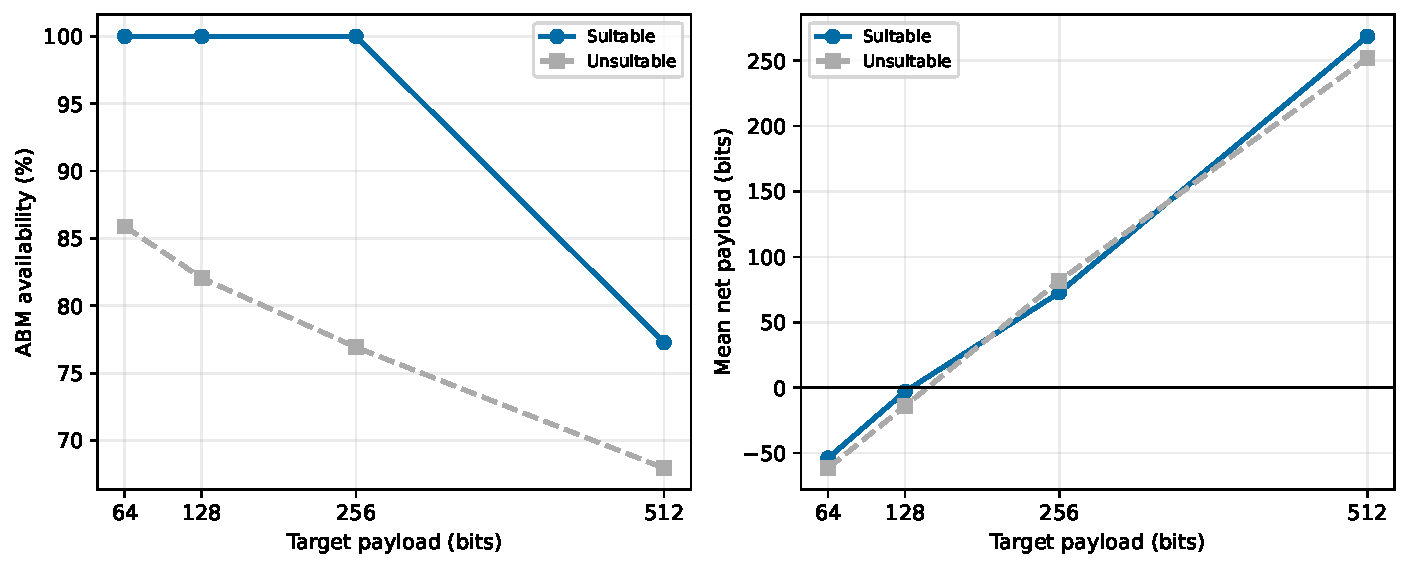
\includegraphics[width=0.92\textwidth]{images/Figure_7.pdf}
\caption{ABM availability and mean net payload after stratification by
fixed-threshold/Otsu agreement.}
\label{fig:binarization}
\end{figure*}

\subsection{Runtime and Memory}

Figure~\ref{fig:resources} and Table~\ref{tab:resources} report the 256-bit
resource benchmark on ten protocol images. PPOCP provides the shortest runtime,
Huynh--Nguyen the smallest incremental memory profile, and ABM requires a
median runtime of 3.56 s and median incremental peak RSS of 2.56 MiB.
Dong's complete ten-divisor optimization
quantifies the computational cost of per-image context search.

\begin{table*}[t]
\centering
\caption{Median resource profile at a 256-bit target.}
\label{tab:resources}
\begin{tabular}{@{}lrrr@{}}
\toprule
\textbf{Method} & \textbf{Available} & \textbf{Time (s)} &
\textbf{Peak RSS increase (MiB)} \\
\midrule
Proposed ABM & 9/10 & 3.56 & 2.56 \\
Dong & 9/10 & 16.97 & 0.05 \\
Huynh--Nguyen & 7/10 & 1.51 & 0.02 \\
PPOCP & 10/10 & 0.16 & 0.70 \\
\bottomrule
\end{tabular}
\end{table*}

Table~\ref{tab:abm-module-runtime} decomposes the proposed method on the eight
document images at the 75\% payload budget. Candidate generation, including
CNN-ranked distance-one assignment, and embedding dominate runtime; the
enumerative serialization itself is negligible.

\begin{table}[t]
\centering
\caption{ABM runtime decomposition by module on document images.}
\label{tab:abm-module-runtime}
\begin{tabular}{@{}lr@{}}
\toprule
\textbf{Module} & \textbf{Median time (s)} \\
\midrule
Candidate generation and ranking & 0.5771 \\
Serialized-prefix optimization & 0.2832 \\
Embedding & 0.7155 \\
Serialization & 0.00015 \\
Extraction & 0.1926 \\
Round-trip verification & 0.00008 \\
\midrule
Total & 1.7857 \\
\bottomrule
\end{tabular}
\end{table}

\begin{figure*}[t]
\centering
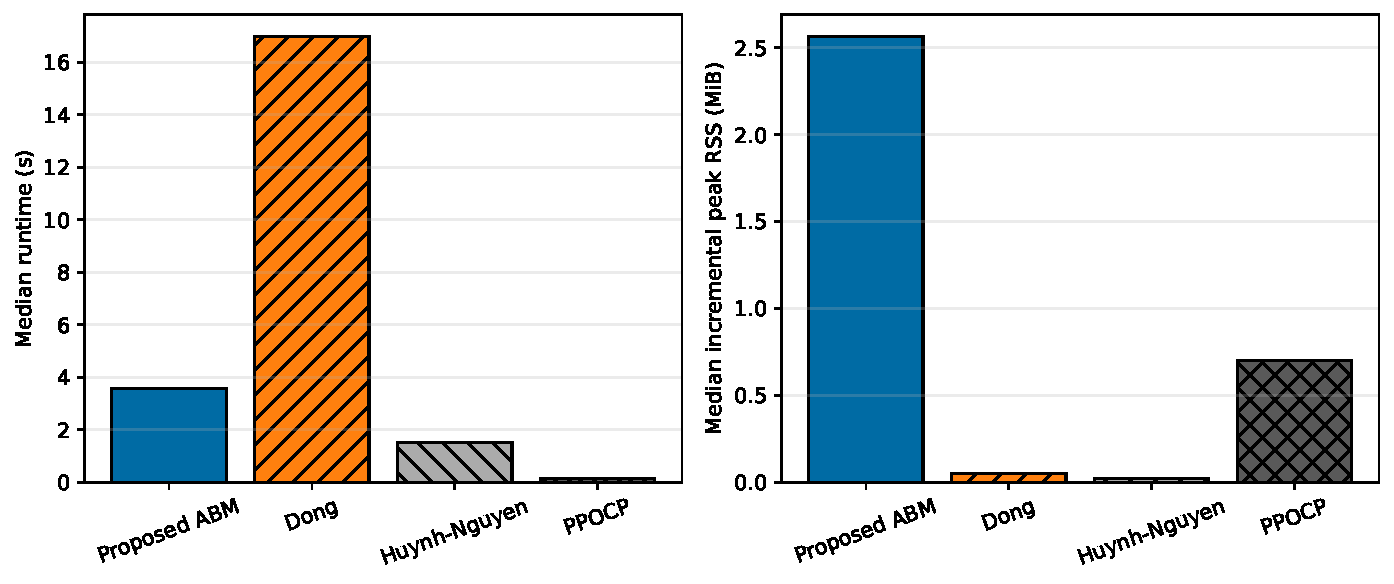
\includegraphics[width=0.92\textwidth]{images/Figure_8.pdf}
\caption{Median wall-clock runtime and incremental peak RSS at 256 bits.}
\label{fig:resources}
\end{figure*}

\subsection{Grouped Steganalysis}
\label{subsec:steganalysis}

The security evaluation uses foreground fraction, horizontal and vertical
transition rates, and normalized $2\times2$ and $3\times3$ pattern histograms.
Five-fold GroupKFold keeps each cover and its stego in the same fold. Both a
standardized logistic model and a 500-tree Random Forest are evaluated.

Figure~\ref{fig:steganalysis} visualizes the complete AUC curves, and
Table~\ref{tab:steganalysis} reports the logistic detector. PPOCP provides the
\RevisionAddBegin
most resistant curve from 128 to 512 bits. ABM's AUC increases with useful
payload, making statistical footprint the principal signal for future
optimization. The Random Forest gives ABM AUC values 0.623, 0.691,
\RevisionAddEnd
0.769, and 0.851, confirming the same payload trend with a different model.
\RevisionAddBegin

A document-image payload sweep explains this trend. When the ABM payload
fraction increases from 25\% to 100\%, mean net payload rises from 329 to 3203
bits, but the mean Jensen--Shannon divergence between cover and marked
$3\times3$ pattern histograms also rises from 0.0087 to 0.0409. Mean
horizontal and vertical transition-rate displacements rise from
0.0032/0.0032 to 0.0127/0.0128. The steganalysis features therefore respond to
the same PEAK/ZERO redistribution that produces useful capacity: repeated PEAK
patterns are depleted and distance-one ZERO patterns are populated. High
payload is therefore best interpreted as capacity-oriented reversible
annotation in access-controlled channels. Figure~\ref{fig:visual-comparison}
gives the qualitative counterpart: residual locations show how each method
distributes its changes under the same 512-bit target on table1-3.
\RevisionAddEnd

\begin{table*}[t]
\centering
\caption{Grouped logistic-detector ROC AUC on matched cover/stego pairs.}
\label{tab:steganalysis}
\begin{tabular}{@{}rccccc@{}}
\toprule
\textbf{Target} & \textbf{Pairs} & \textbf{Proposed ABM} &
\textbf{Dong} & \textbf{Huynh--Nguyen} & \textbf{PPOCP} \\
\midrule
64  & 86 & 0.706 & 0.656 & \textbf{0.599} & 0.653 \\
128 & 83 & 0.826 & 0.759 & 0.688 & \textbf{0.654} \\
256 & 69 & 0.900 & 0.784 & 0.774 & \textbf{0.691} \\
512 & 46 & 0.957 & 0.896 & 0.909 & \textbf{0.690} \\
\bottomrule
\end{tabular}
\end{table*}

\begin{figure*}[t]
\centering
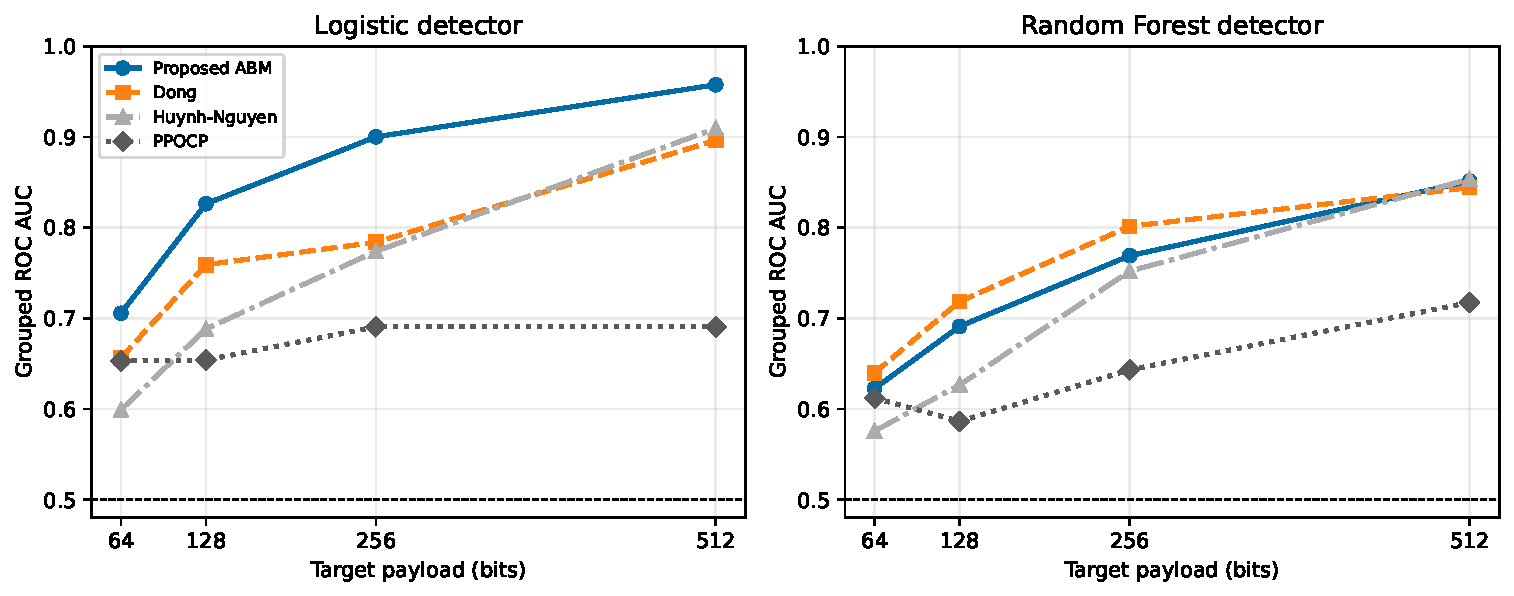
\includegraphics[width=\textwidth]{images/Figure_9.pdf}
\caption{Grouped steganalysis across payloads with logistic (left) and Random
Forest (right) detectors. The dashed line denotes chance-level AUC.}
\label{fig:steganalysis}
\end{figure*}

\begin{figure*}[t]
\centering
\begin{minipage}{0.49\textwidth}
\centering
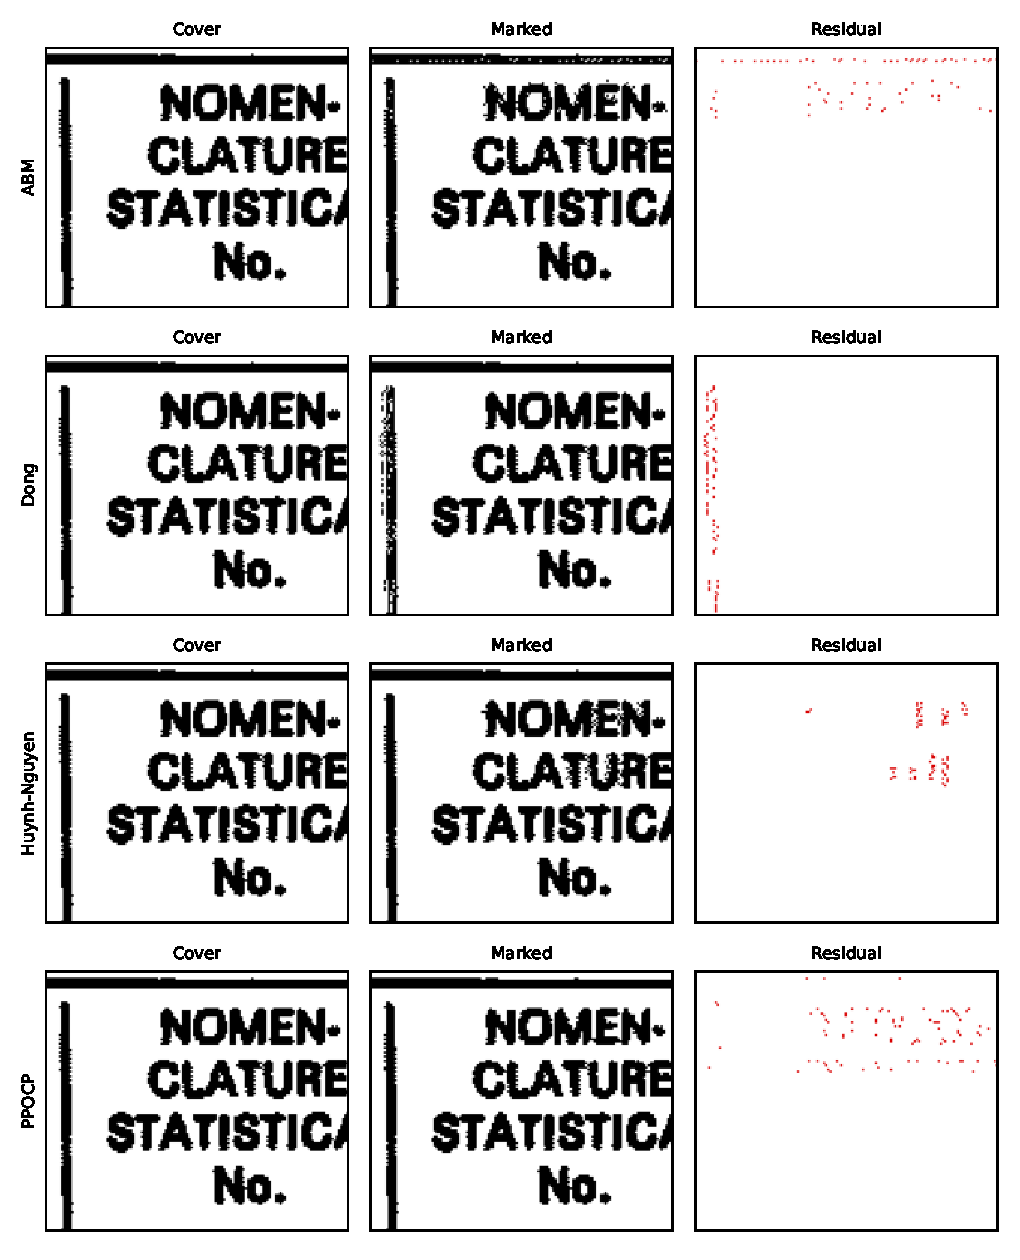
\includegraphics[width=\linewidth,trim=0 300bp 0 0,clip]{images/Figure_10.pdf}
\end{minipage}\hfill
\begin{minipage}{0.49\textwidth}
\centering
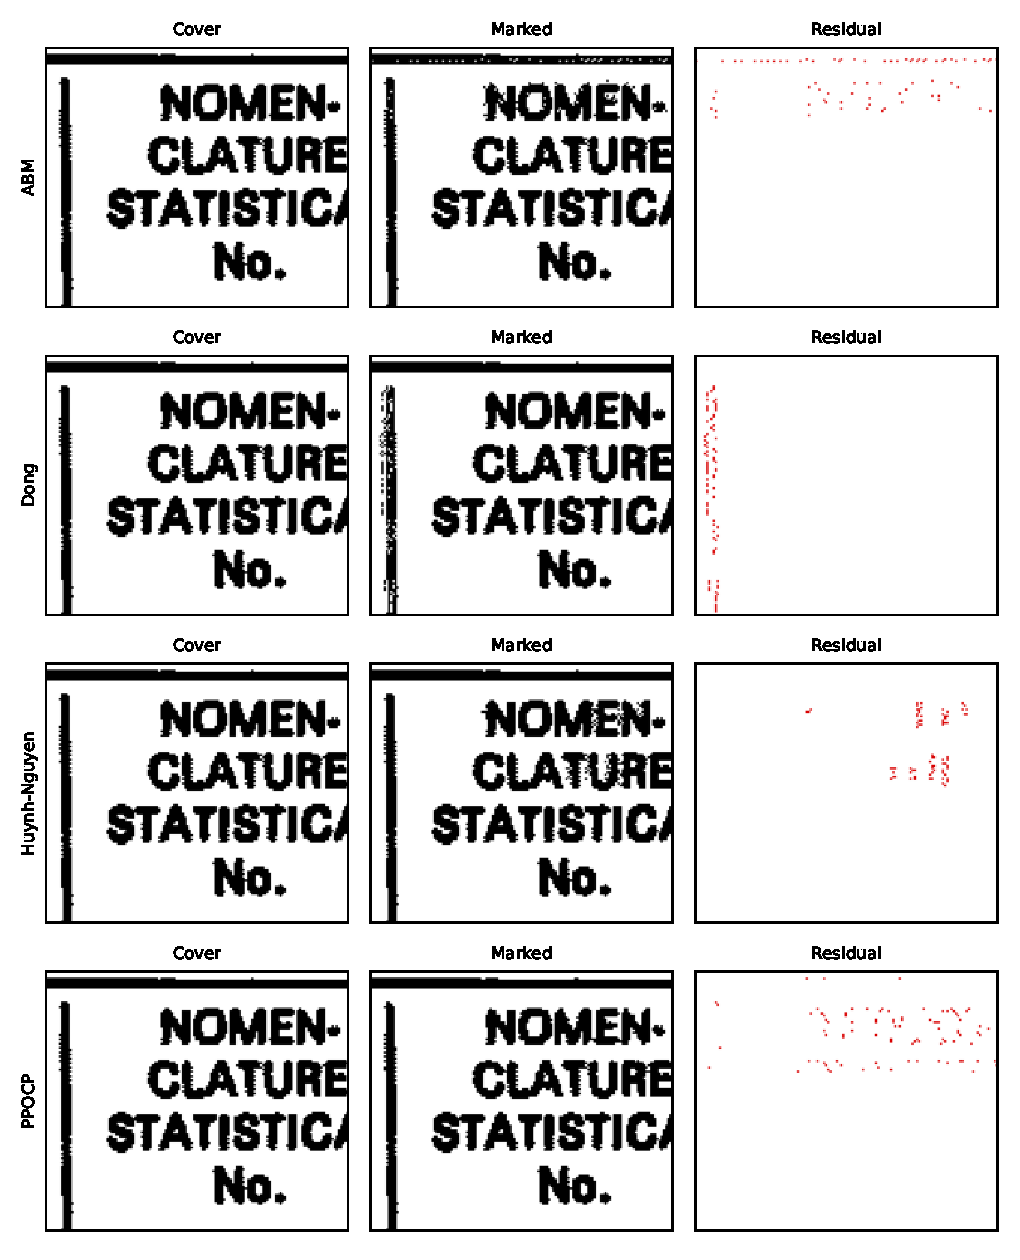
\includegraphics[width=\linewidth,trim=0 0 0 325bp,clip]{images/Figure_10.pdf}
\end{minipage}
\caption{Cover, marked, and residual zooms on table1-3 at a 512-bit target,
split into two panels to fit the two-column layout: ABM and Dong appear on the left, and
Huynh--Nguyen and PPOCP on the right. Residual pixels are
shown in red on the marked crop to make modification locations visible under
the same payload.}
\label{fig:visual-comparison}
\end{figure*}

\section{Discussion}
\label{sec:discussion}

\subsection{Positioning Across Practical Objectives}

The experiments separate four objectives that are frequently merged in RDH
\RevisionAddBegin
comparisons. In useful capacity, ABM provides the highest net-payload curve and
crosses into mean-positive net payload between 128 and 256 bits. In
\RevisionAddEnd
perceptual quality, PPOCP defines the lowest median DRD, followed closely by
Huynh--Nguyen at the higher target. In applicability, PPOCP has universal
target availability, while ABM combines high availability with compact side
information. In computational cost, ABM remains practical and is substantially
faster than the complete Dong parameter search.

This decomposition supports a specific, protocol-bounded position: among the
four evaluated implementations, ABM provides the highest net payload after
serialized metadata, whereas PPOCP provides the lowest-distortion and
\RevisionAddBegin
most favorable detectability profile. This conclusion rests on exact round trips,
\RevisionAddEnd
multi-payload curves, a fixed-cohort sensitivity analysis, and paired tests.
Because synchronization formats materially affect net payload, the result is
\RevisionAddBegin
framed as a protocol-bounded comparison of the evaluated implementations.
\RevisionAddEnd

\subsection{Security-Aware Optimization Direction}

\RevisionAddBegin
The measured AUC curves and content-adaptive detectability principles
\cite{Sedighi2018Content} suggest a direct route for strengthening the method.
The current CNN predicts reciprocal-distance cost, whereas the steganalysis
\RevisionAddEnd
features respond to shifts in local pattern distributions. A security-aware
ranker can optimize
\begin{equation}
\mathcal{L}(Z_j)=
\beta\,\widehat{\mathrm{DRD}}(Z_j)
+\gamma\,\Delta_{\mathrm{hist}}(Z_j)
+\eta\,\Delta_{\mathrm{trans}}(Z_j),
\label{eq:security-aware-ranker}
\end{equation}
where $\Delta_{\mathrm{hist}}$ measures the change in local pattern histograms
and $\Delta_{\mathrm{trans}}$ measures transition-rate displacement. The
coefficients can be selected on a Pareto front of net bits, DRD, and grouped
detector AUC. This extension builds directly on the validated ranker and
preserves the exact reversible wire format.

\RevisionAddBegin
The present measurements define the operating envelope. At 256 and
512 bits, logistic AUC values of 0.900 and 0.957 place the current ABM
configuration in a capacity-oriented reversible-annotation regime, despite its
positive net payload and exact reversibility. At 64 bits, AUC 0.706 reflects
lower detectability, although metadata overhead dominates useful capacity.
PPOCP remains the
\RevisionAddEnd
preferred evaluated method for security-prioritized operation, whereas ABM
addresses applications in which useful reversible capacity is primary and
the stego channel itself is access-controlled.

\RevisionAddBegin
The RF uniform-block experiment points to a second optimization path:
\RevisionAddEnd
coordinate coding can use enumerative subset coding conditioned on the
deterministic block order. Its grouped classification metrics show that
location selection is reliable; compressing the selected subset targets the
measured source of overhead.

\subsection{Experimental Scope}
\label{subsec:scope}

The eight document images provide continuity with the binary block-mapping
literature, and the disjoint BOSSbase protocol adds 100 external test images,
four payloads, paired inference, resources, and steganalysis. BOSSbase
\RevisionAddBegin
binarization should be read as a transfer test, with a large scanned document
corpus remaining a natural next benchmark. The 512-bit all-method cohort
contains 46 images, so both
\RevisionAddEnd
availability and fixed-cohort results are reported. The logistic AUC of 0.957
at that payload identifies a high-order statistical footprint even though the
\RevisionAddBegin
visual DRD remains moderate. These measured boundaries define the validated
\RevisionAddEnd
operating region and provide explicit targets for distribution-aware ranking.
The reversible channel assumes lossless storage and transmission. A stress test
on table1-3 at 256 bits confirms exact recovery after PNG and TIFF round trips,
while JPEG recompression at quality 5 and one-pixel perturbation convert the
input into mismatched stego/auxiliary pairs, illustrating the required
lossless-channel assumption (Table~\ref{tab:channel-stress}). Geometric,
noisy, or lossy transformations therefore require an external synchronization
or error-control layer.

\begin{table}[t]
\centering
\caption{Channel stress test for ABM with the same auxiliary stream.}
\label{tab:channel-stress}
\begin{tabular}{@{}lccc@{}}
\toprule
\textbf{Channel} & \textbf{Stego} &
\textbf{Message} & \textbf{Cover} \\
\midrule
PNG & Yes & Yes & Yes \\
TIFF & Yes & Yes & Yes \\
JPEG q=5 & Altered & Mismatch & Mismatch \\
One-pixel noise & Altered & Mismatch & Mismatch \\
\bottomrule
\end{tabular}
\end{table}

\section{Conclusion}
\label{sec:conclusion}

\RevisionAddBegin
This work develops and evaluates serialization-aware activation for
net-payload-driven PEAK/ZERO block mapping in binary-image RDH. The
enumerative codec makes the active mapping description executable and charged;
the CNN ranker improves candidate placement on held-out images as a secondary
cost-ordering component. The complete system delivers 2245 net bits on average
on eight document images and 292.5 net bits on 100 BOSSbase images. Every
reported available experiment restores the message and cover exactly.
\RevisionAddEnd

Under the common protocol, ABM obtains mean net payloads of $-57$, $-7$, $93$,
and $309$ bits at targets 64, 128, 256, and 512 bits on matched images. Its
paired net advantage is significant against every baseline after Holm
correction; at 256 bits, all adjusted $p$-values are below
\RevisionAddBegin
$6.7\times10^{-13}$. Together, availability, binarization, runtime, memory,
and two-classifier steganalysis make this result a reproducible practical
profile beyond a single capacity number.
\RevisionAddEnd

Under the stated implementations and wire-level accounting, the combined
\RevisionAddBegin
evidence identifies ABM as the highest useful-capacity curve in the evaluated
common protocol, while PPOCP retains the lowest measured distortion and most
favorable detectability profile. This evidence therefore adds a concrete
net-capacity benchmark and an
\RevisionAddEnd
exactly reversible reference implementation. The measured security curves
\RevisionAddBegin
also identify local-distribution preservation as the main optimization
\RevisionAddEnd
target while retaining compact metadata and exact restoration.

\section*{Acknowledgements}
\RevisionAddBegin
This work was supported by the authors' institutions.
\RevisionAddEnd

\printcredits

\section*{Declarations}
\noindent\textbf{Ethics approval.}
This study does not involve human participants, animals, personal data, or
clinical interventions. It uses publicly available image data and offline
computational experiments.

\medskip
\noindent\textbf{Competing interests.}
The authors declare that they have no known competing financial interests or
\RevisionAddBegin
personal relationships that could have appeared to influence the work reported
in this paper.
\RevisionAddEnd

\medskip
\noindent\textbf{Funding.}
This research received no external funding.

\medskip
\noindent\textbf{Data availability.}
BOSSbase is publicly available from its original distributor at
\url{https://dde.binghamton.edu/download/ImageDB/BOSSbase_1.01.zip} under its
applicable terms. The eight document images used for block-mapping validation,
derived aggregate results, and per-image evaluation artefacts accompany the
reproducibility package.

\medskip
\noindent\textbf{Code availability.}
The reproducibility package contains the ABM implementation, independently
implemented comparison methods, evaluation scripts, tests, trained model
weights, CSV/JSON result tables, plotting code, and exact random seeds. It is
publicly available at
\url{https://github.com/EkodeckStephane/net-aware-block-mapping-rdh}.

\bibliographystyle{cas-model1-num-names}
\bibliography{references}

\end{document}
